\chapter{Section 3}
\section{Summary of the Situation After the First Assignment}
\subsection{Dashboard} \label{dashboard}
In the preceding report, no version incorporating any 
of the panel members was presented. 
\begin{figure}[H]
    \centerline{%
    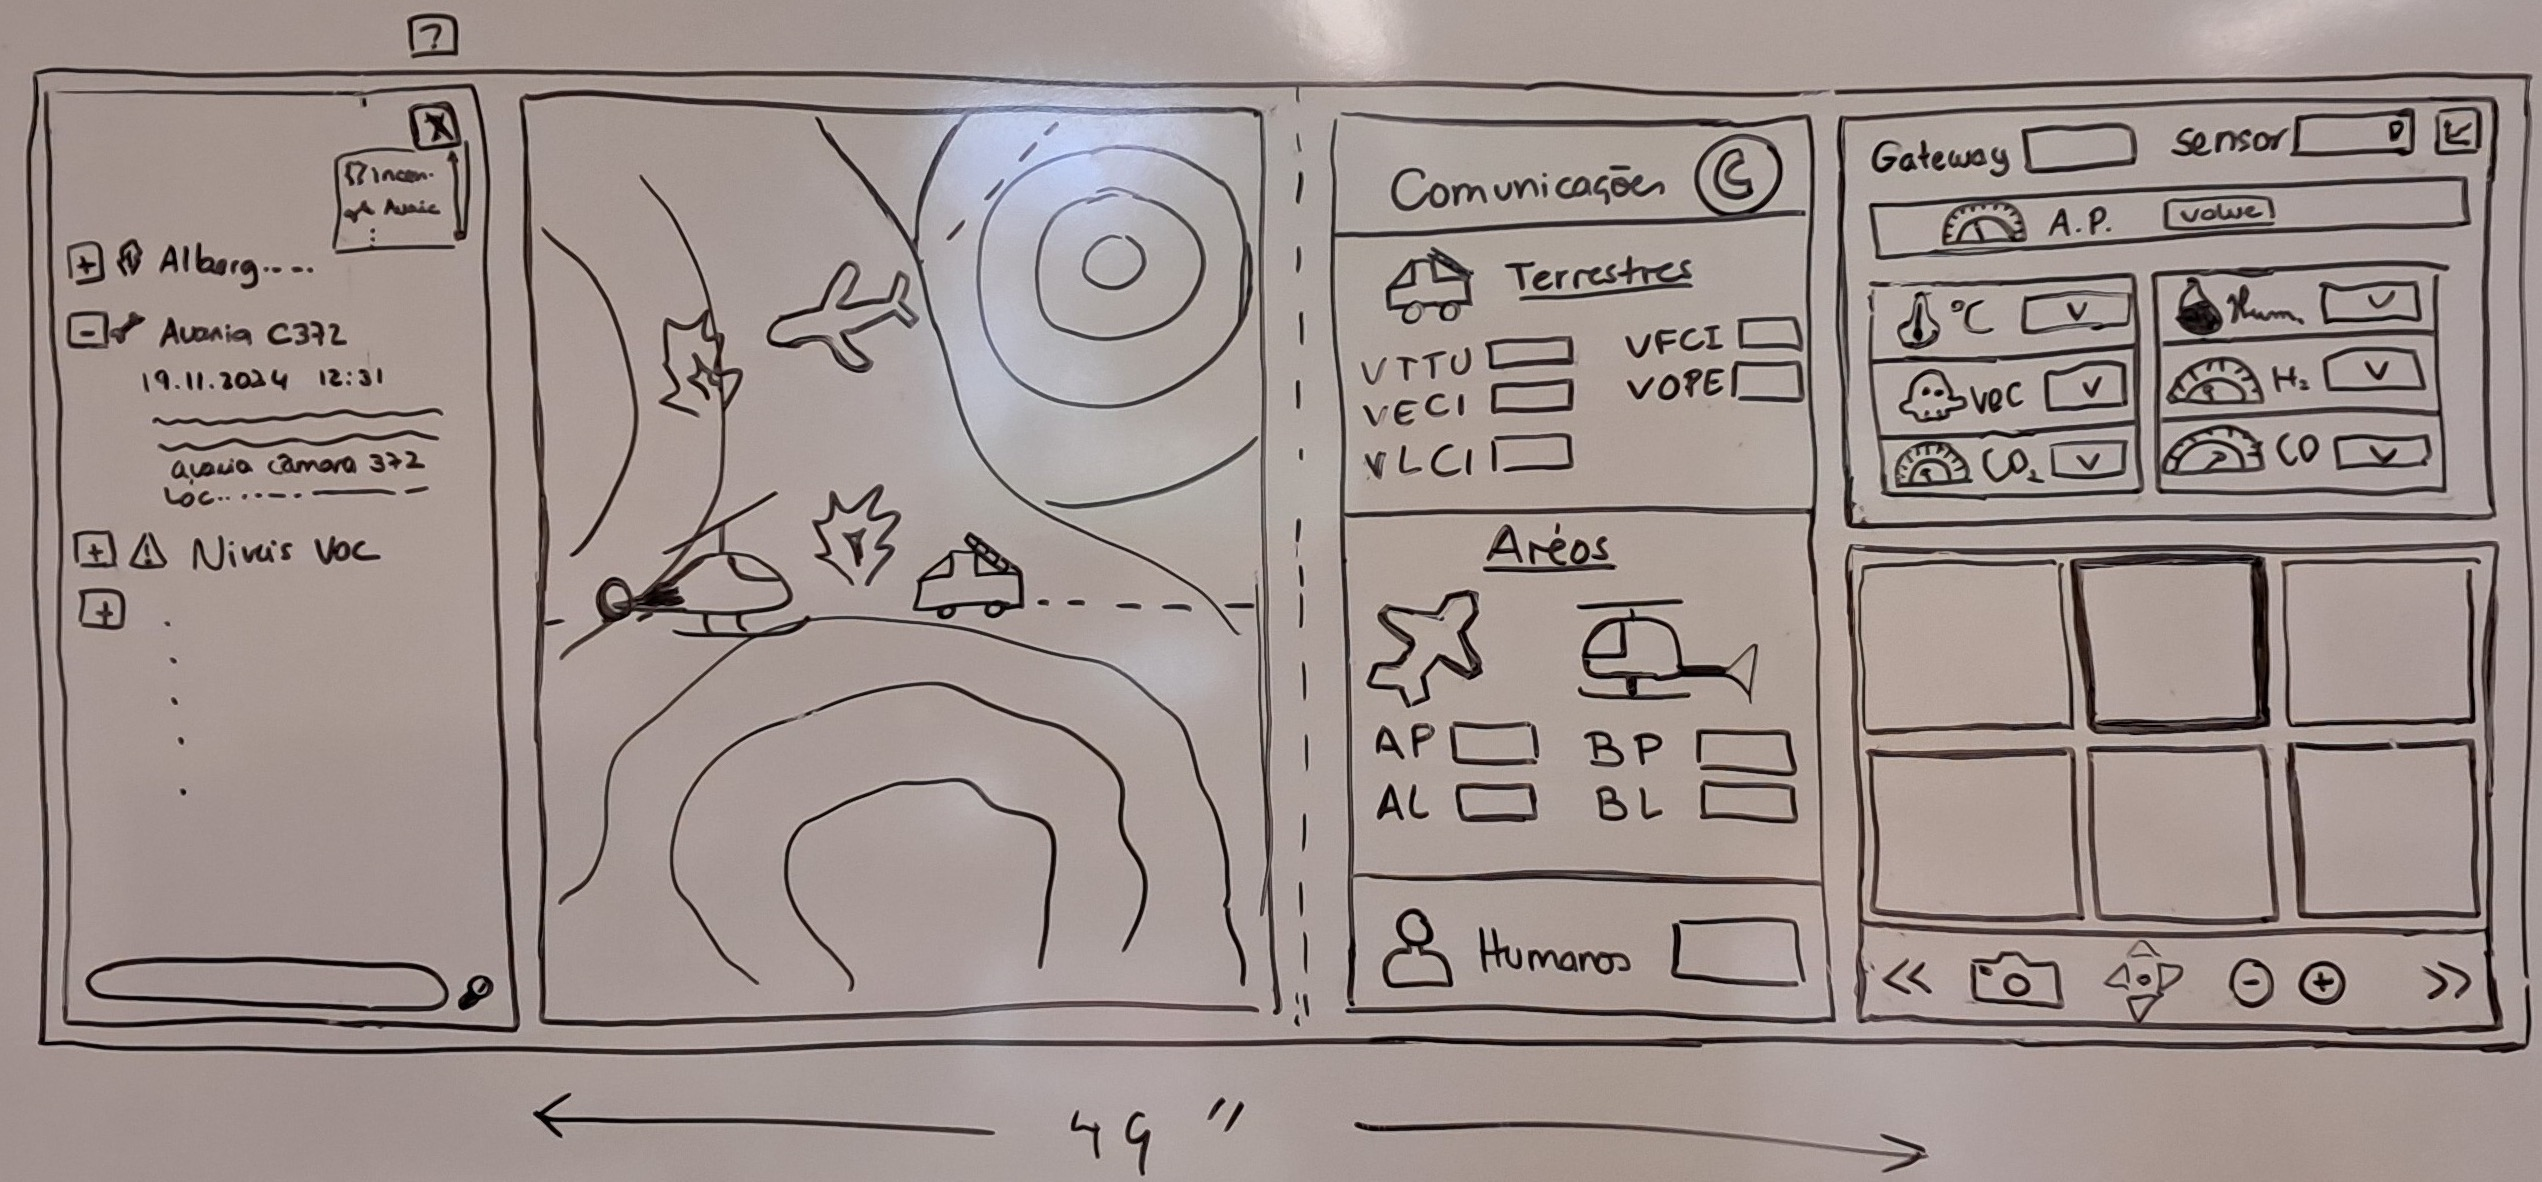
\includegraphics[width=\textwidth]{20241119_134559 (1).jpg}
    %
    }
    \caption{Dashboard}
\end{figure}
\section{Detected Problems and Sketches in Low Fidelity}
Some sketches were hard to understand, particularly 
some of the Cameras Panel sketches, like sketch 3. 
\section{Visual Features}
\subsection{Choice of Color Palette}
In order to create a colour palette for use in the 
prototype, the Coolors software (\url{https://coolors.co/}) was employed. Initially, 
19 colour palettes were generated (named palettes, 
where x was the number between 1-8, 10-17 and 19-21), 
which are presented beneath. \par 
\begin{figure}[H]
    \centerline{%
    \subfloat[Palette 1]{
        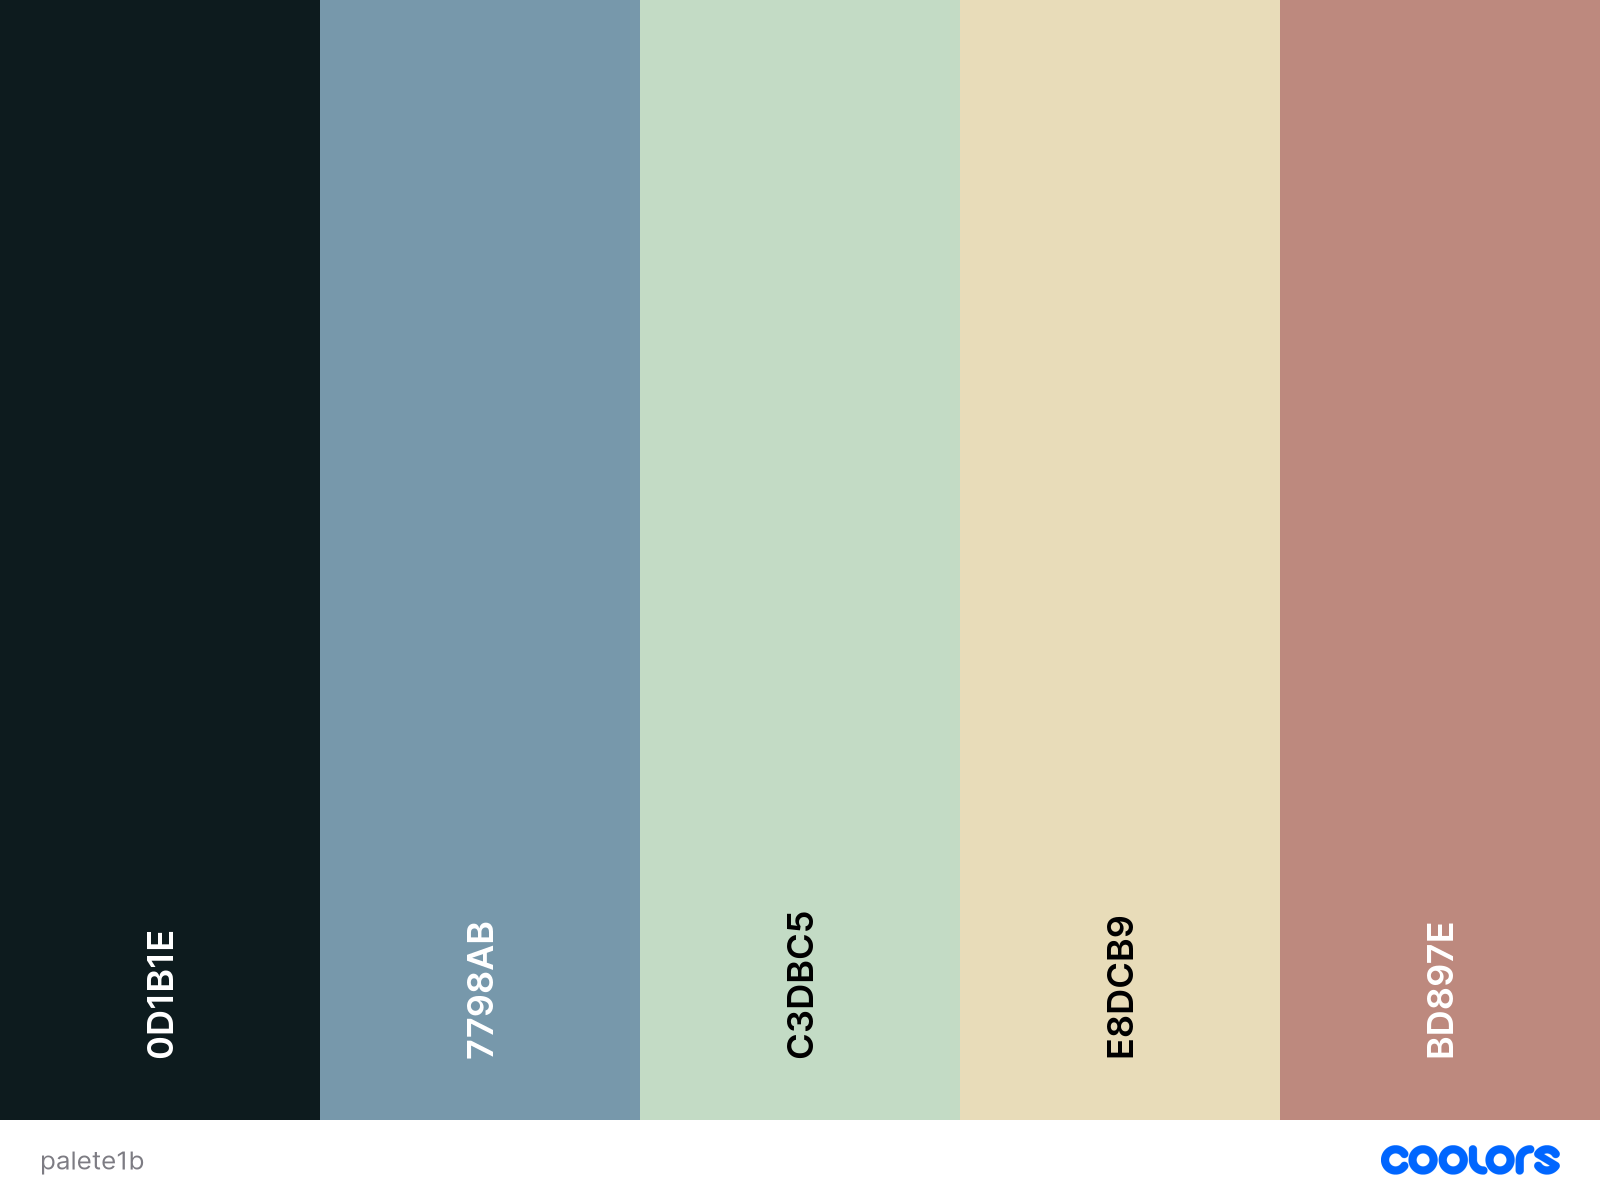
\includegraphics[width=.33\textwidth]{palete1.png}
    }\hfill
    \subfloat[Palette 2]{
        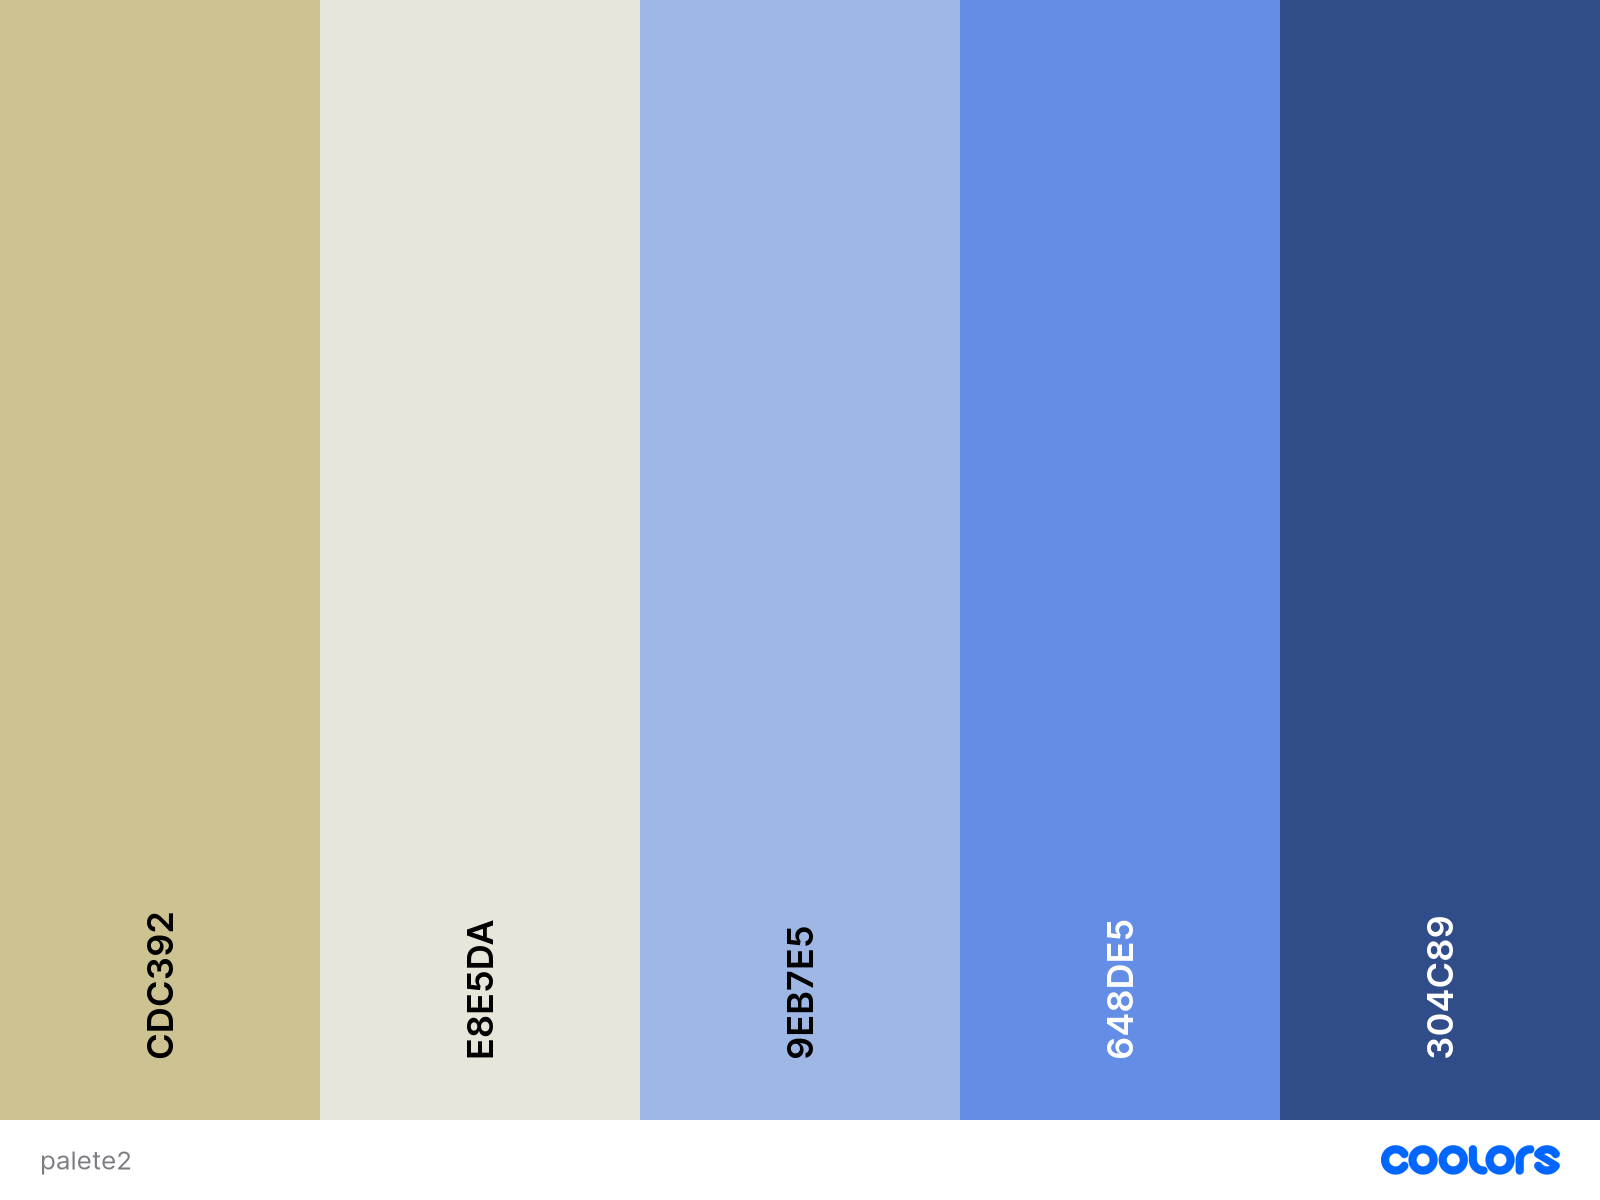
\includegraphics[width=.33\textwidth]{palete2.png}
    }\hfill
    \subfloat[Palette 3]{
        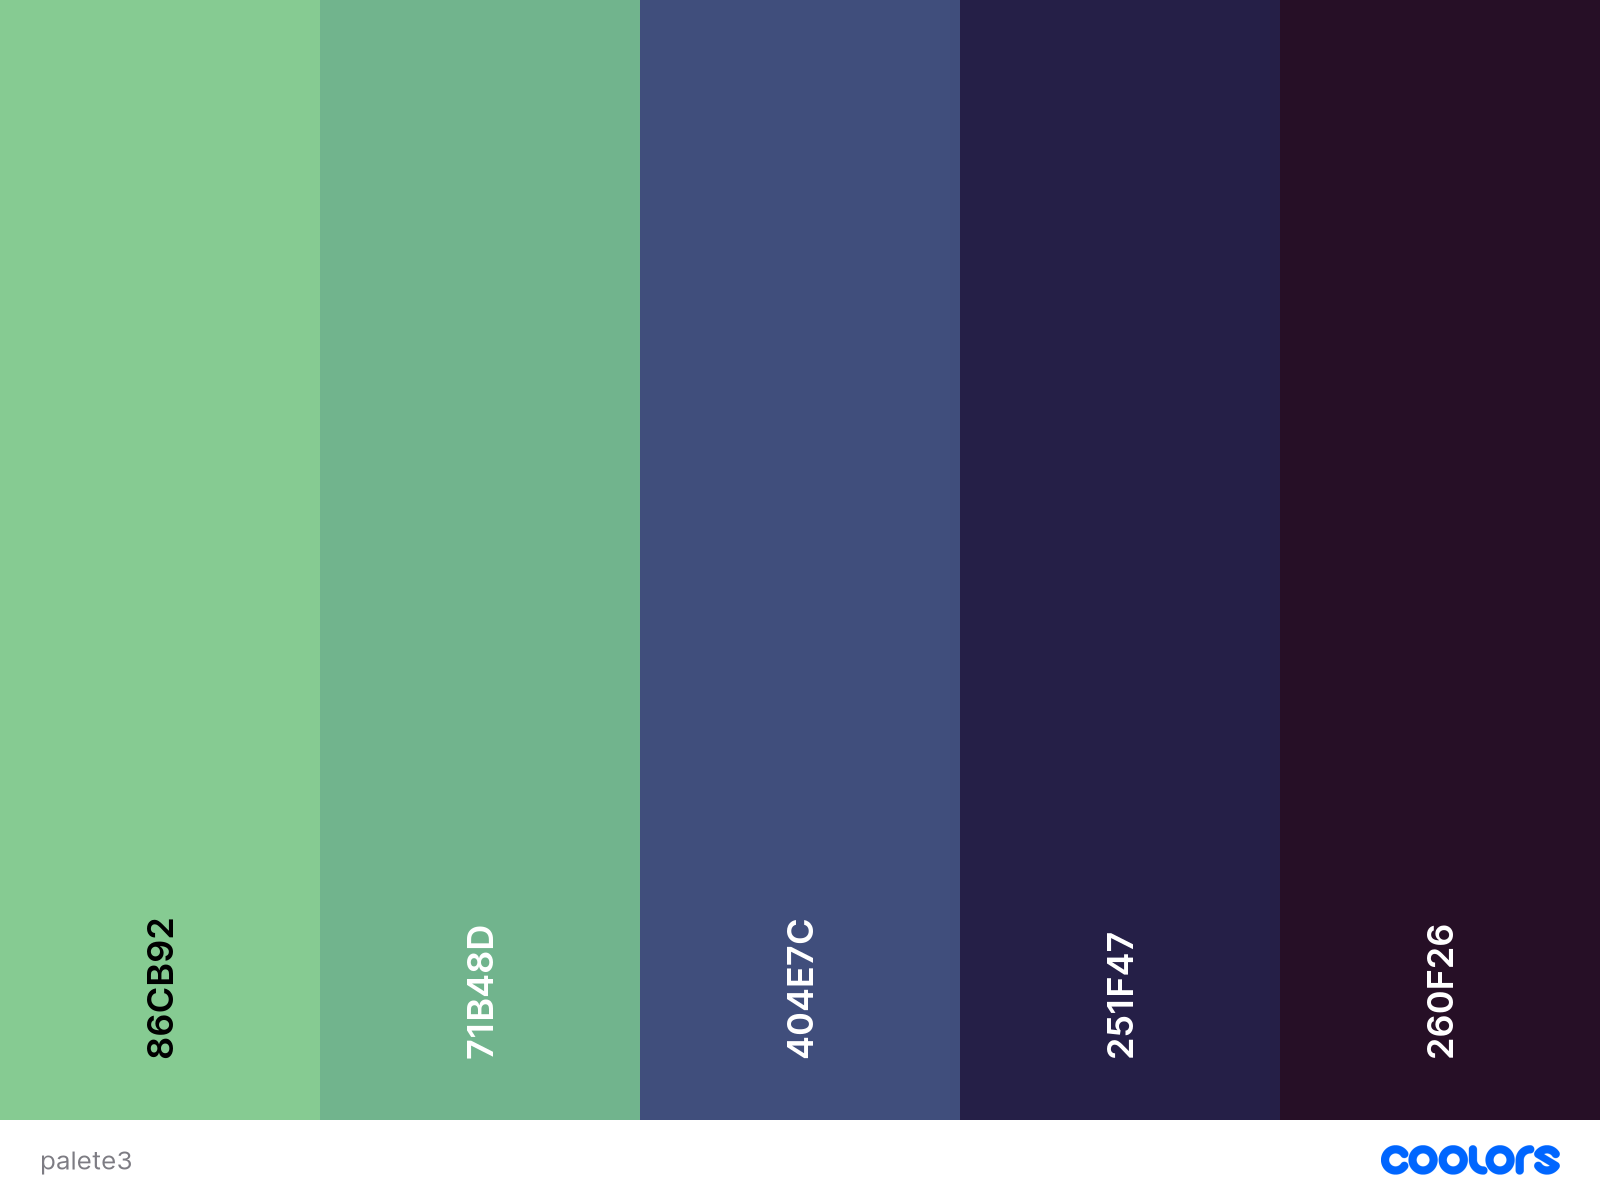
\includegraphics[width=.33\textwidth]{palete3.png}
    }
    %
    }
    \centerline{%
    \subfloat[Palette 4]{
        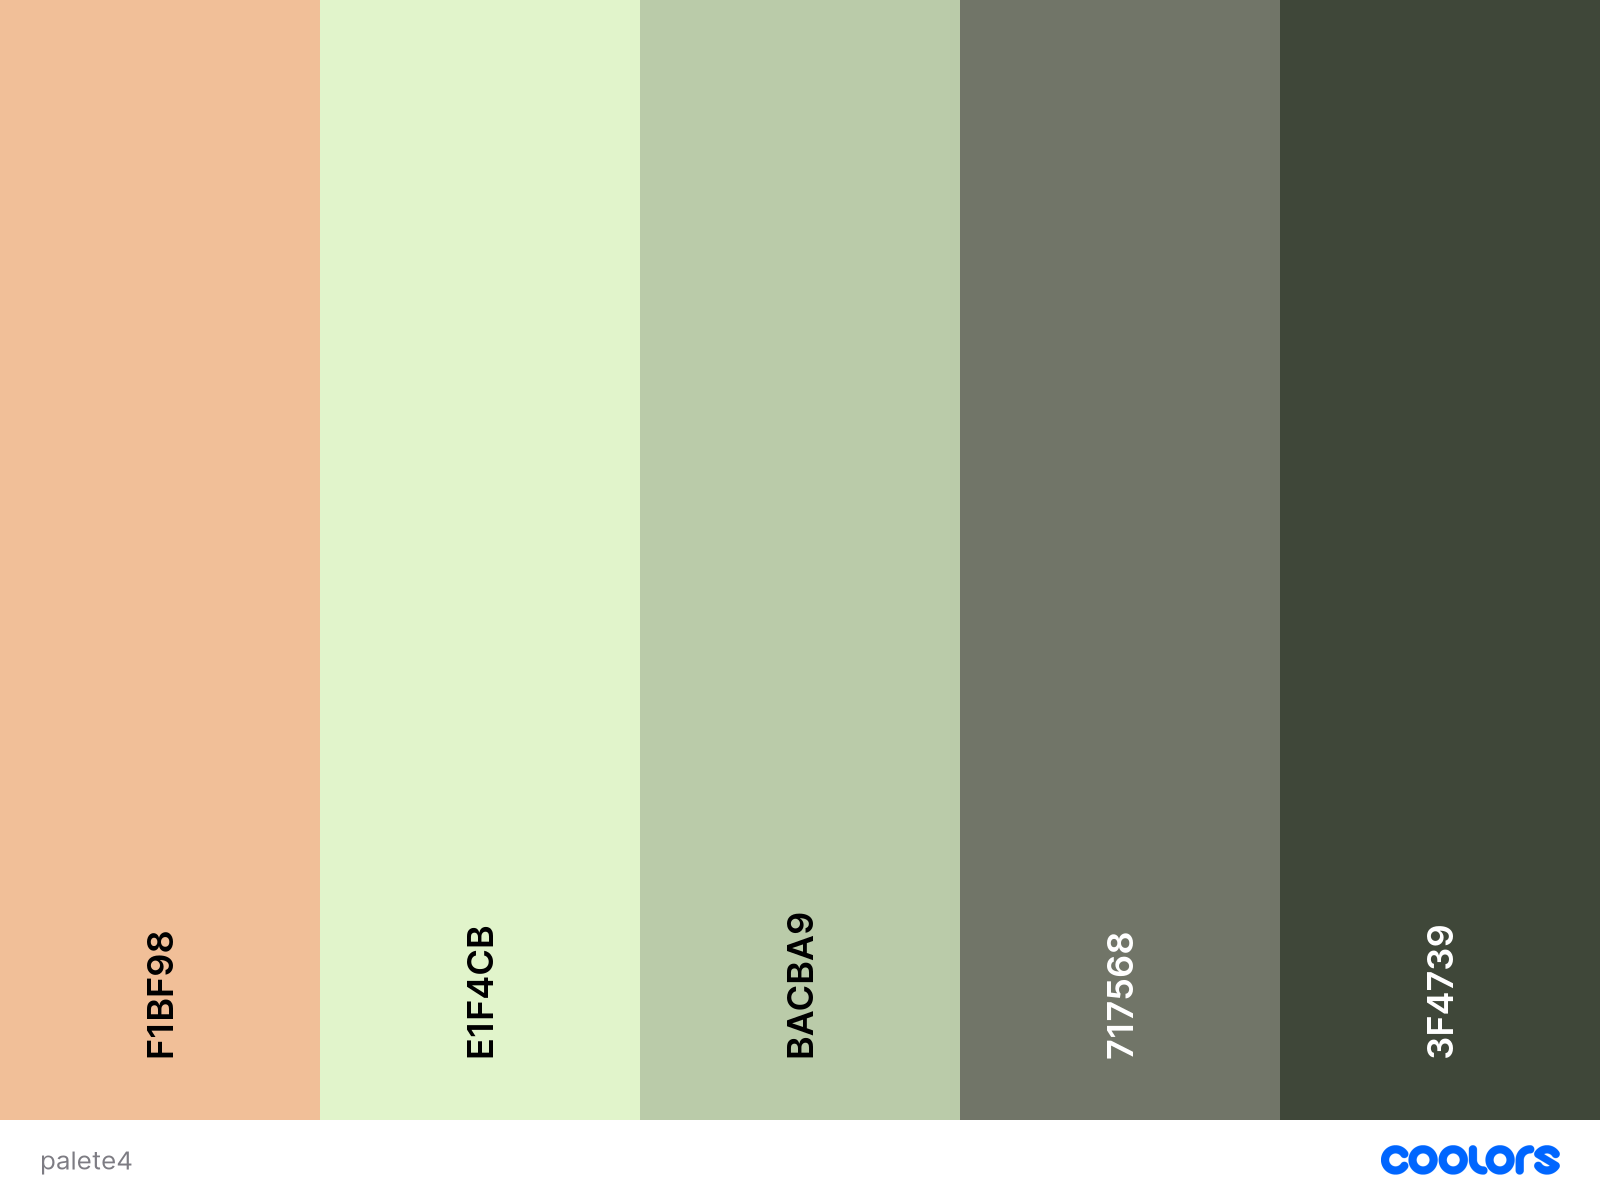
\includegraphics[width=.33\textwidth]{palete4.png}
    }\hfill
    \subfloat[Palette 5]{
        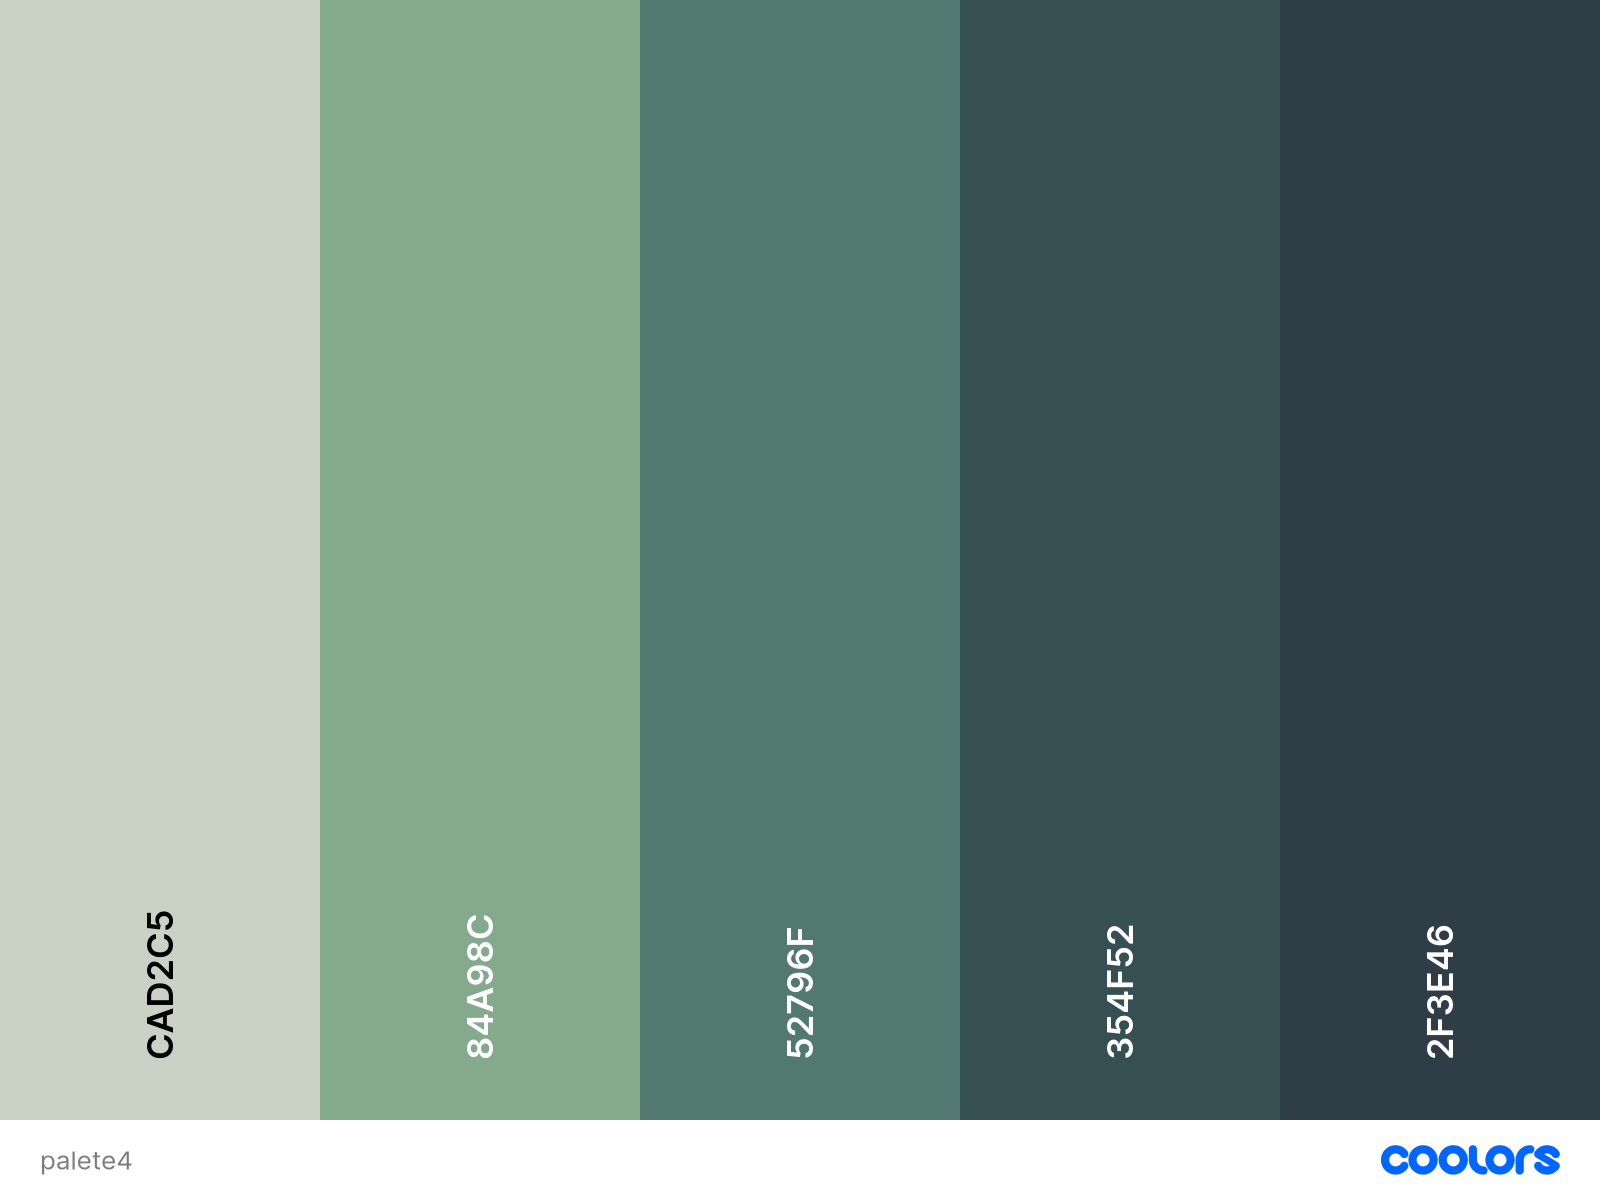
\includegraphics[width=.33\textwidth]{palete5.png}
    }\hfill
    \subfloat[Palette 6]{
        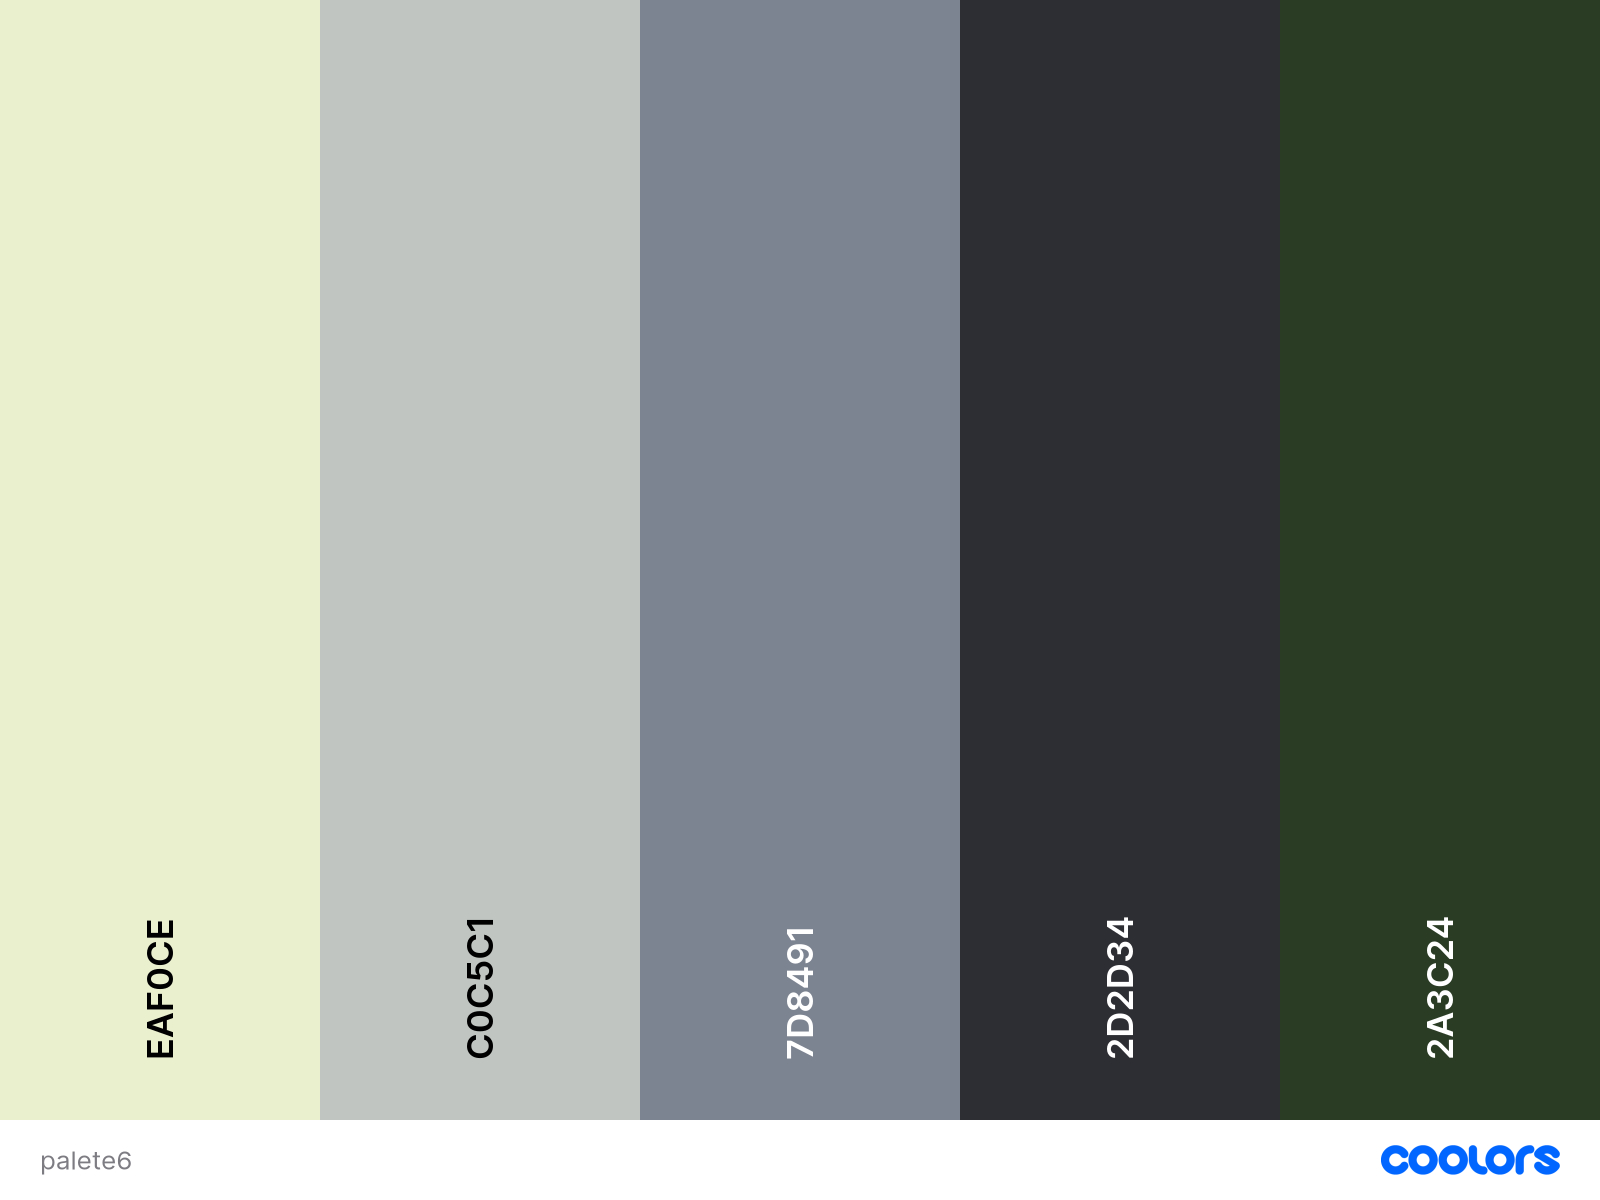
\includegraphics[width=.33\textwidth]{palete6.png}
    }%
    }
%\end{figure}
%\begin{figure}[H]\ContinuedFloat
    \centerline{%
    \subfloat[Palette 7]{
        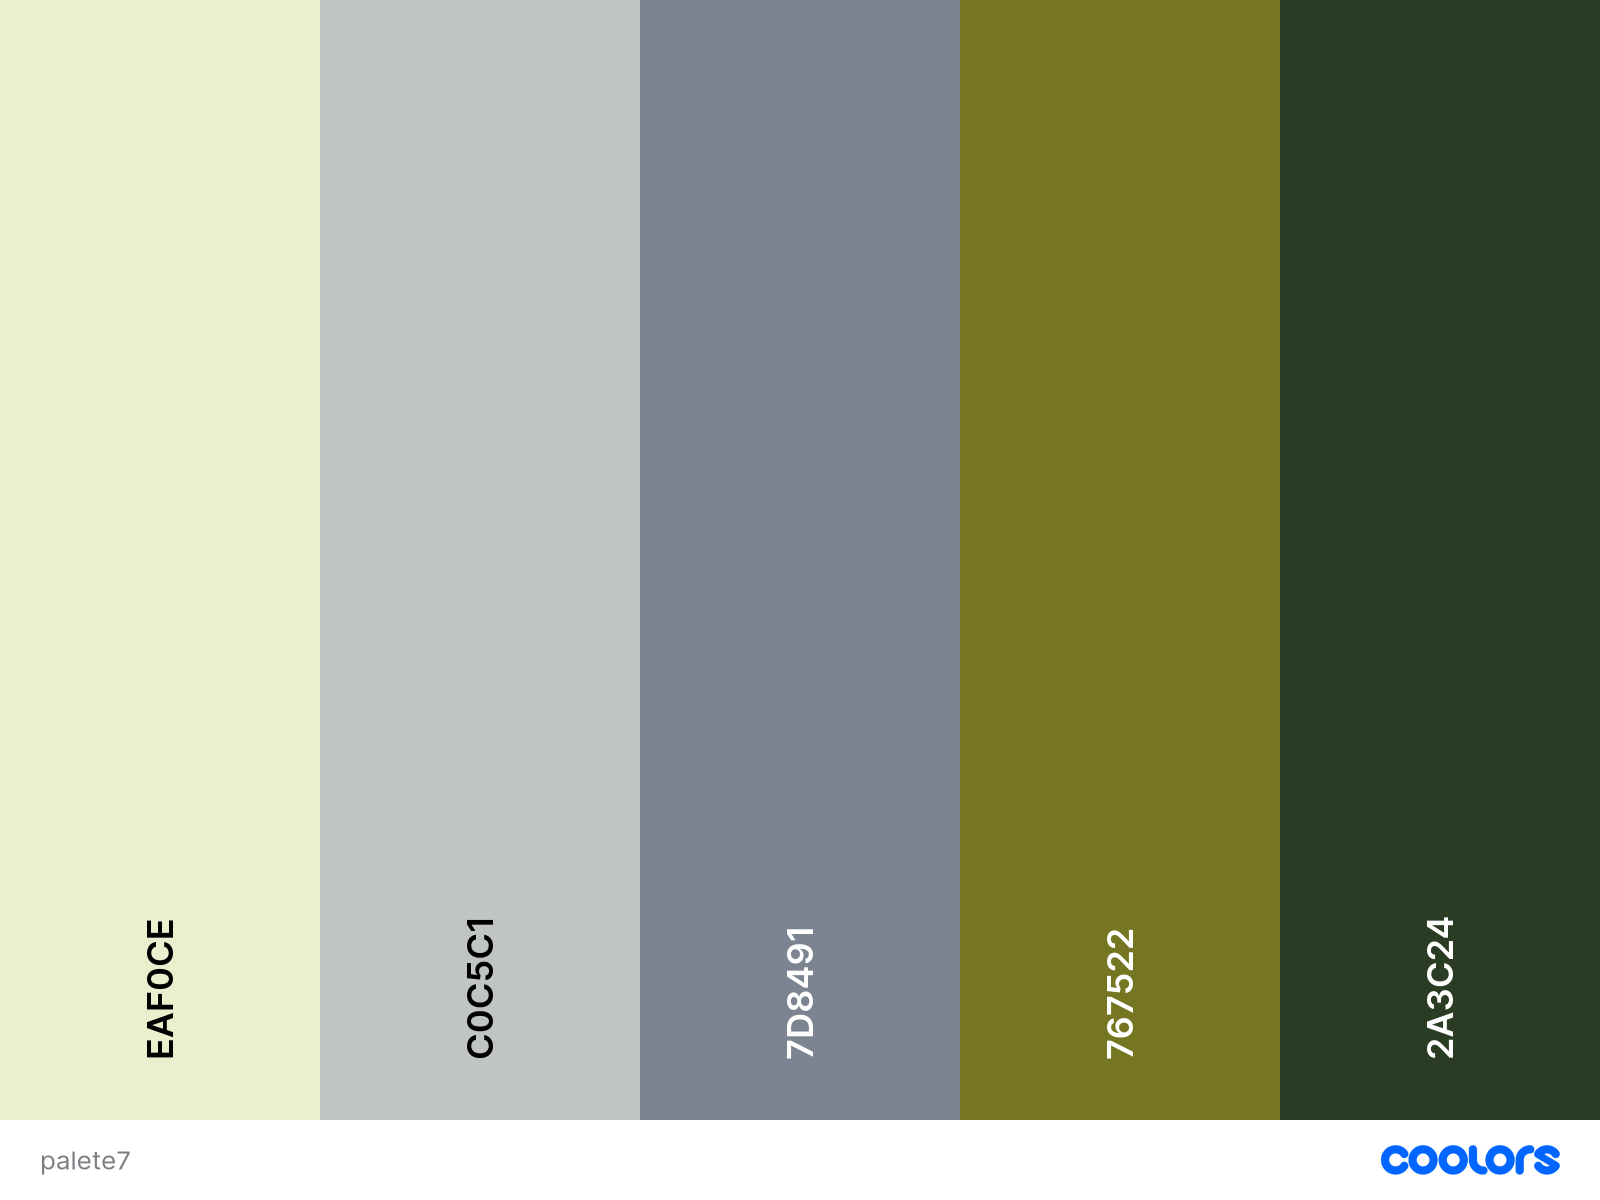
\includegraphics[width=.33\textwidth]{palete7.png}
    }\hfill
    \subfloat[Palette 8]{
        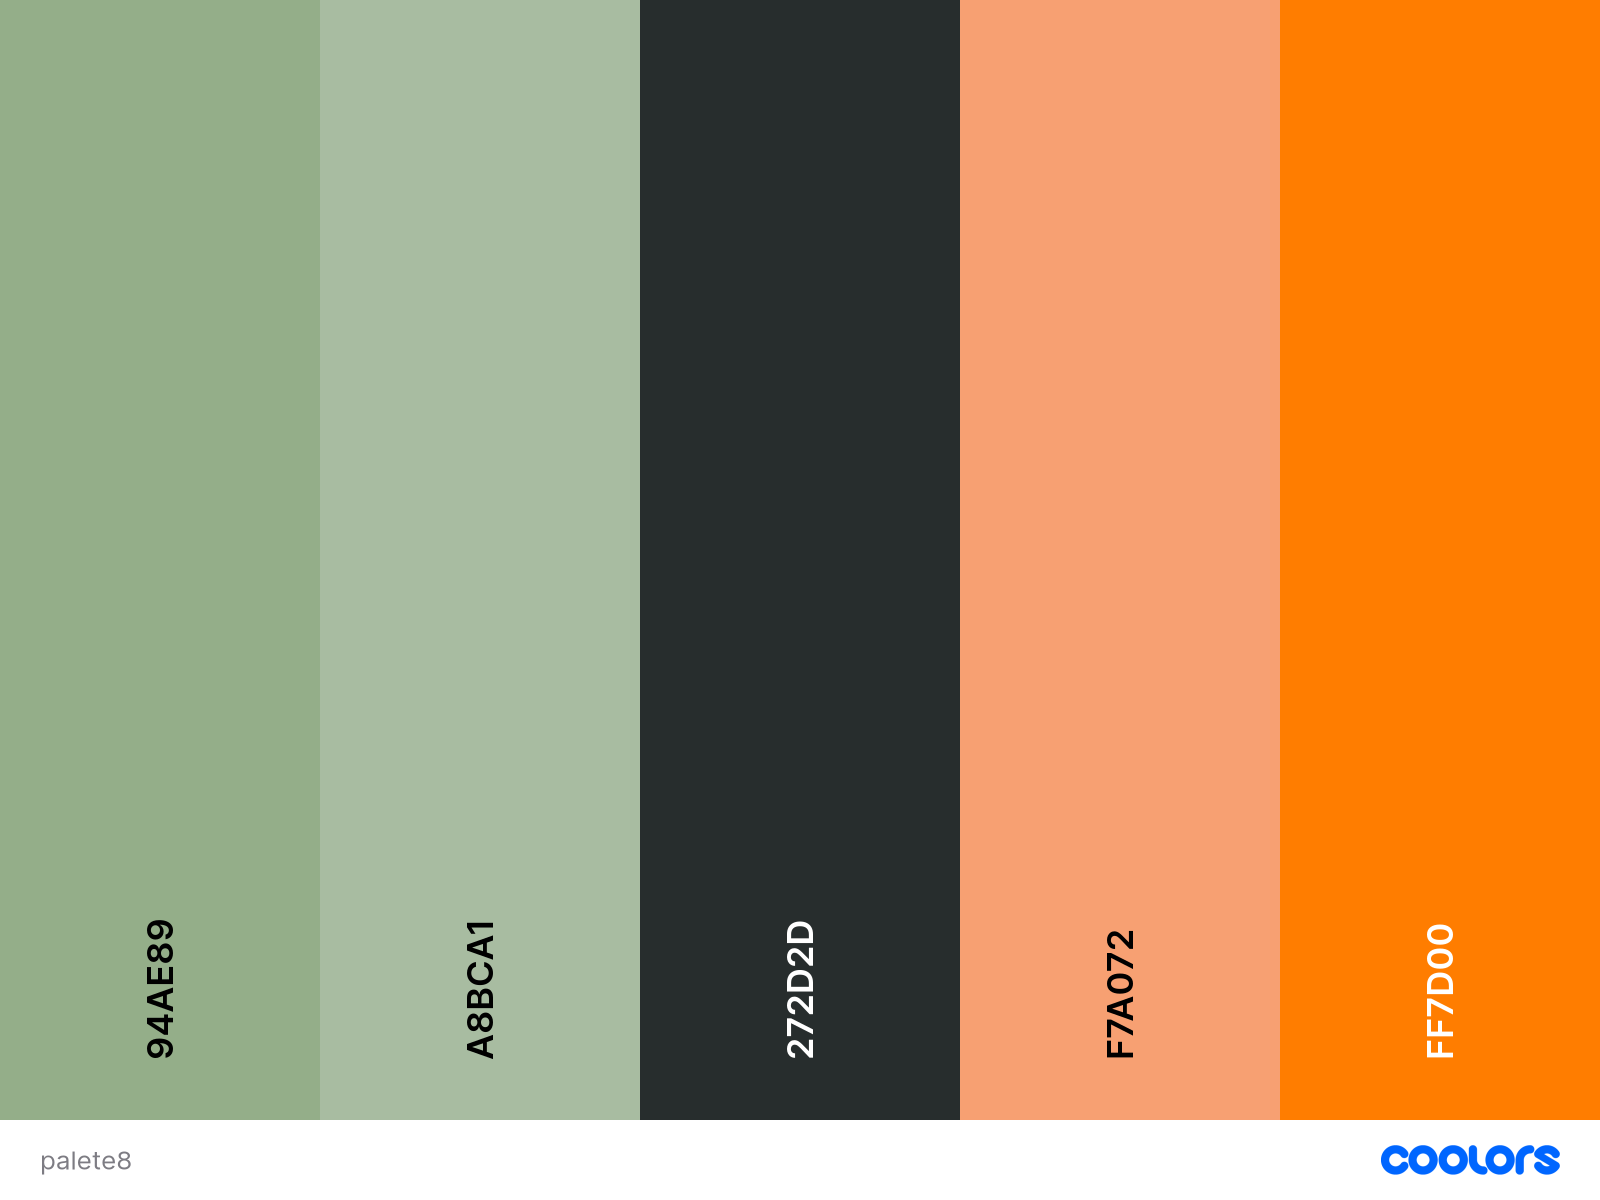
\includegraphics[width=.33\textwidth]{palete8.png}
    }\hfill
    \subfloat[Palette 10]{
        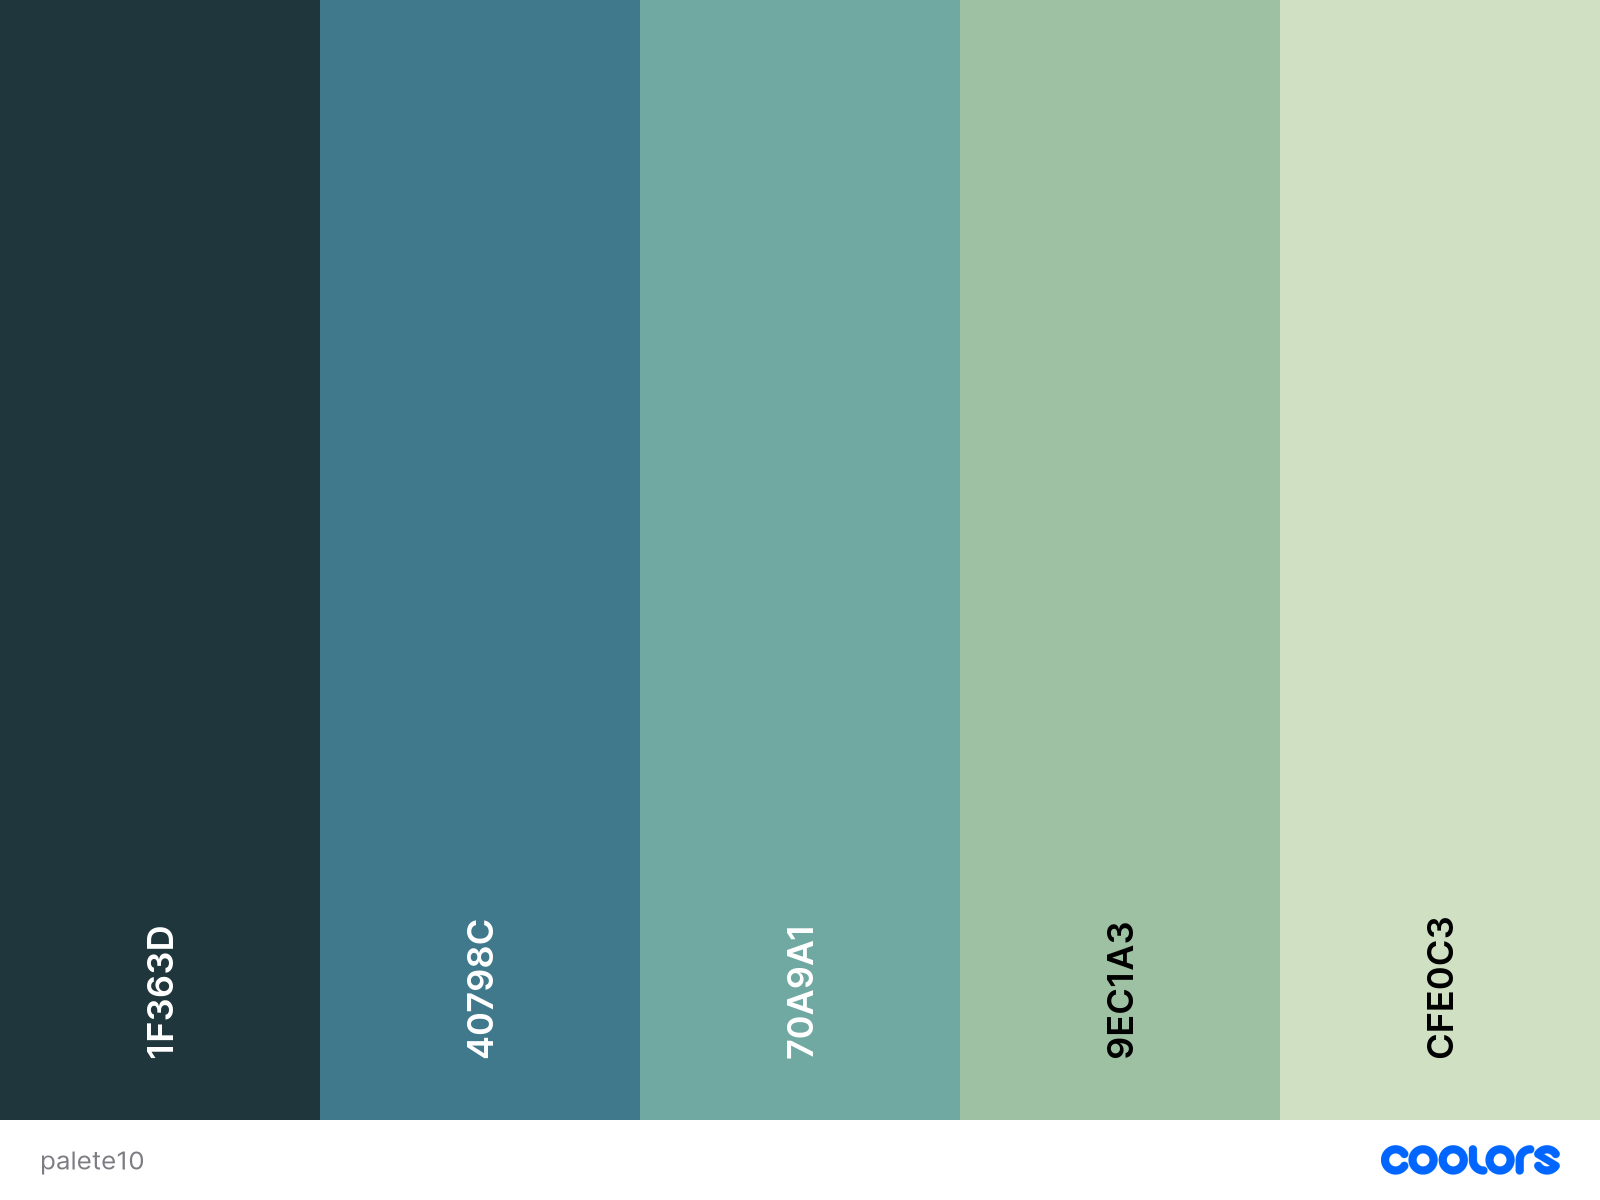
\includegraphics[width=.33\textwidth]{palete10.png}
    }%
    }
    \centerline{%
    \subfloat[Palette 11]{
        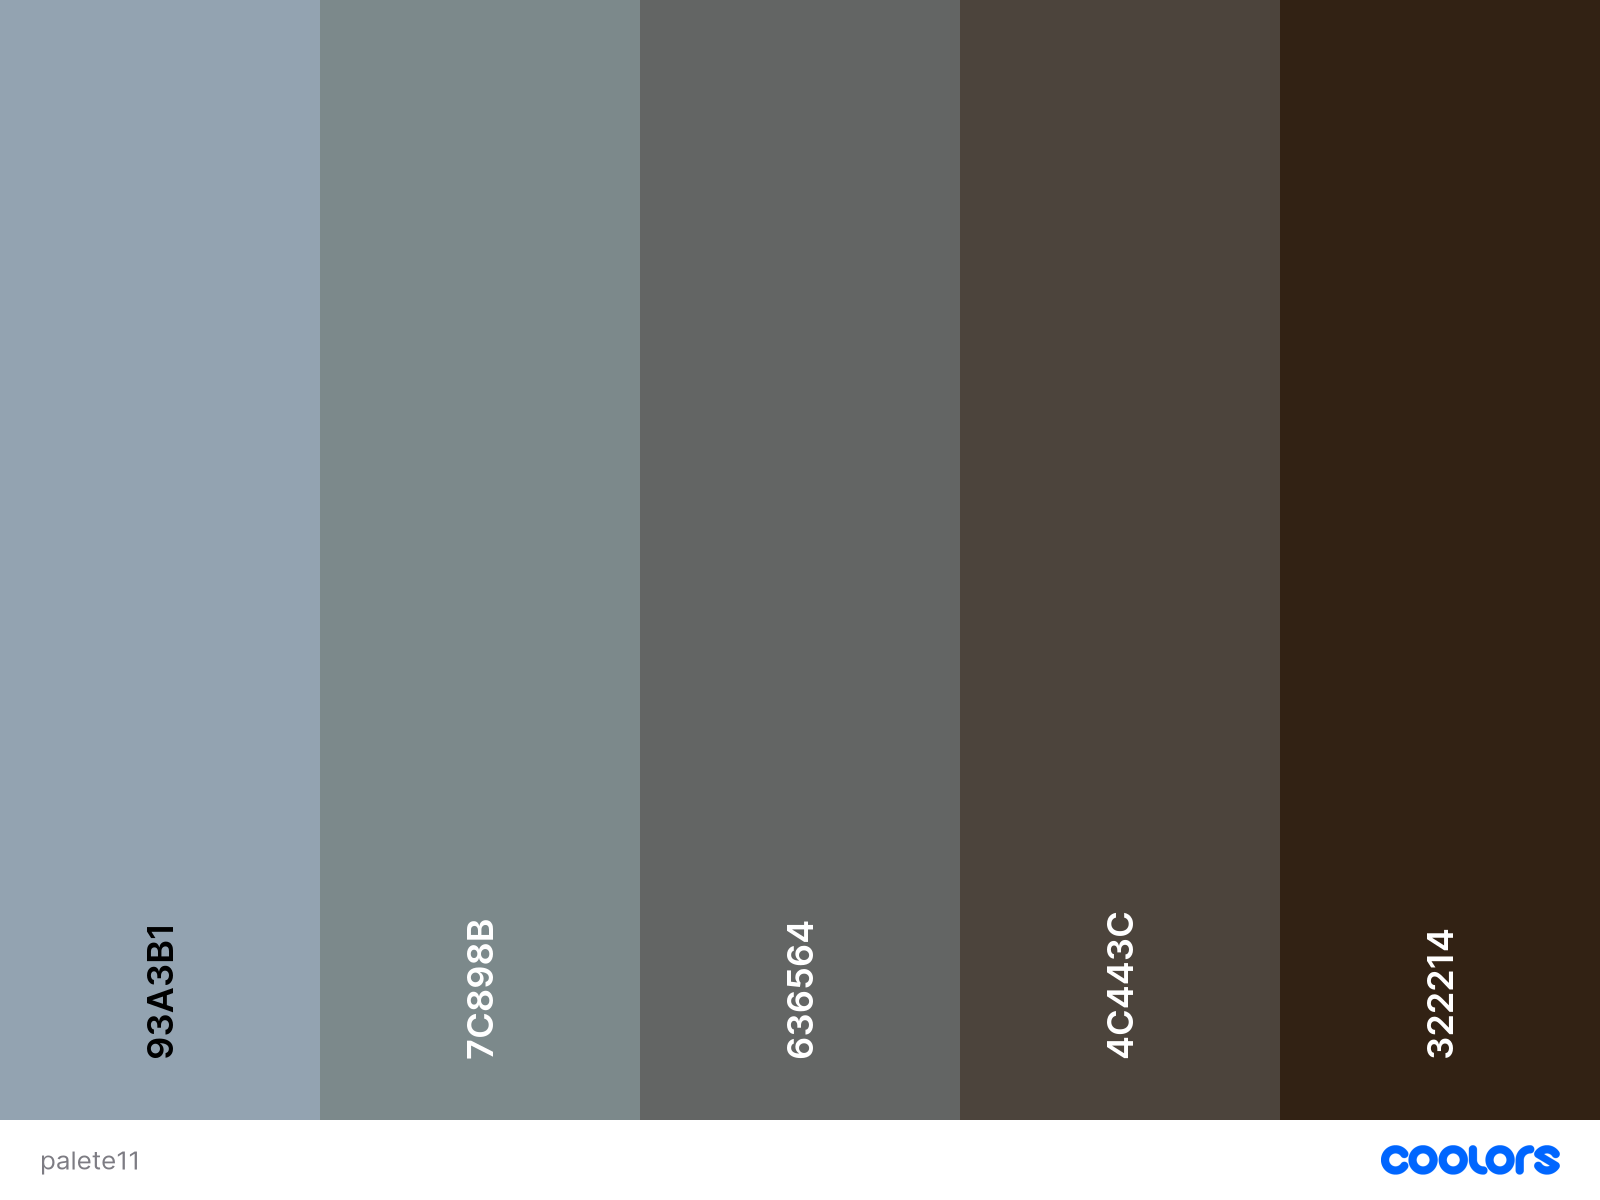
\includegraphics[width=.33\textwidth]{palete11.png}
    }\hfill
    \subfloat[Palette 12]{
        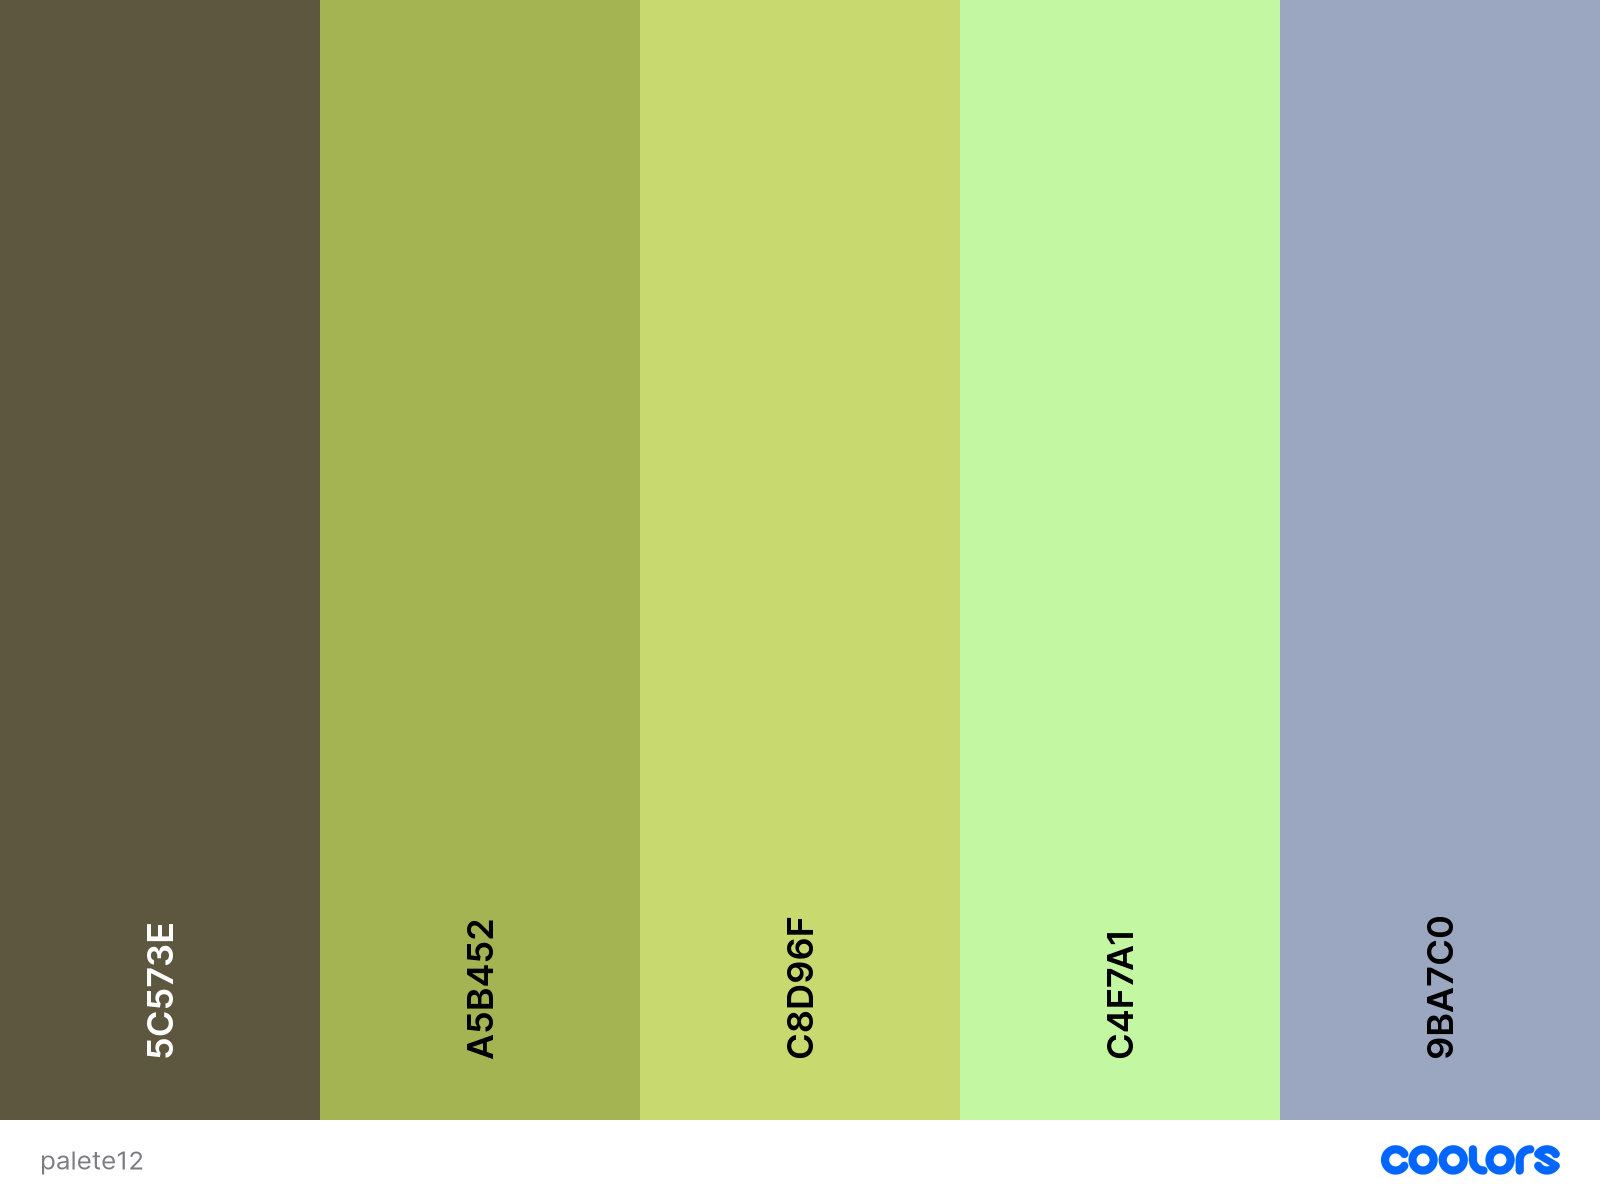
\includegraphics[width=.33\textwidth]{palete12.png}
    }\hfill
    \subfloat[Palette 13]{
        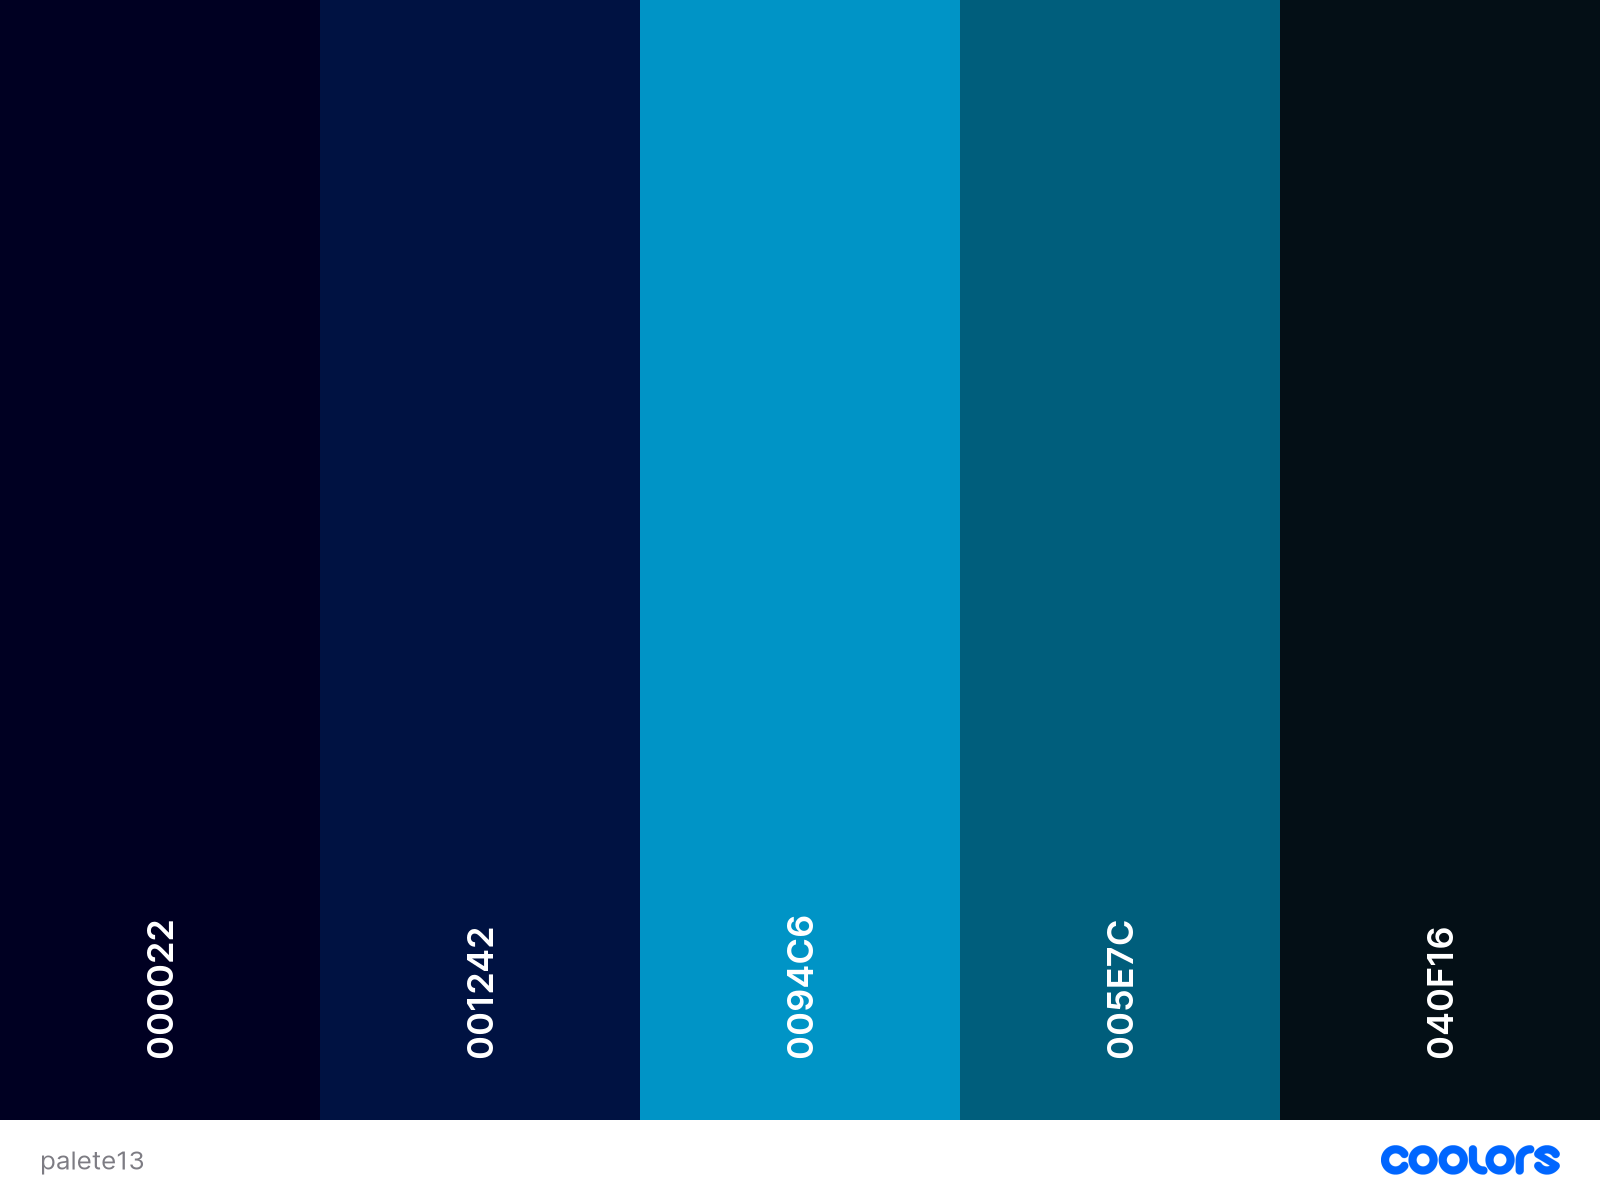
\includegraphics[width=.33\textwidth]{palete13.png}
    }%
    }
    \centerline{%
    \subfloat[Palette 14]{
        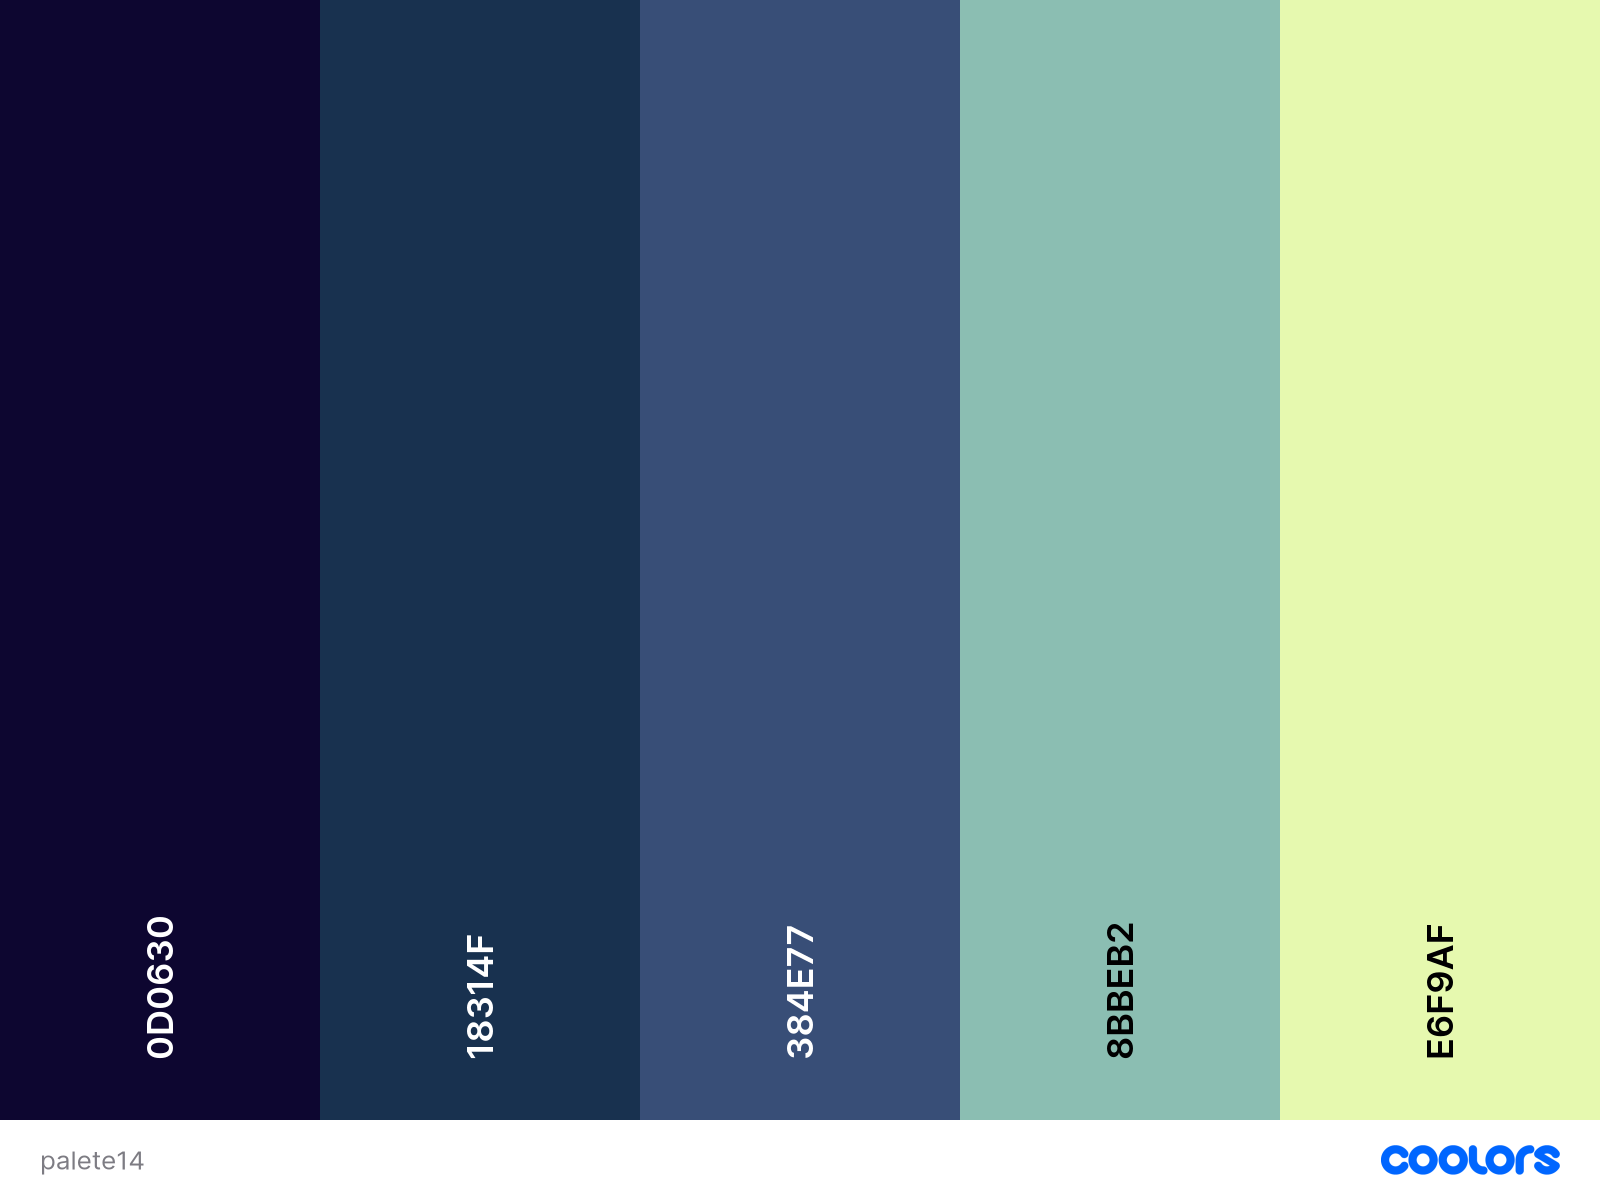
\includegraphics[width=.33\textwidth]{palete14.png}
    }\hfill
    \subfloat[Palette 15]{
        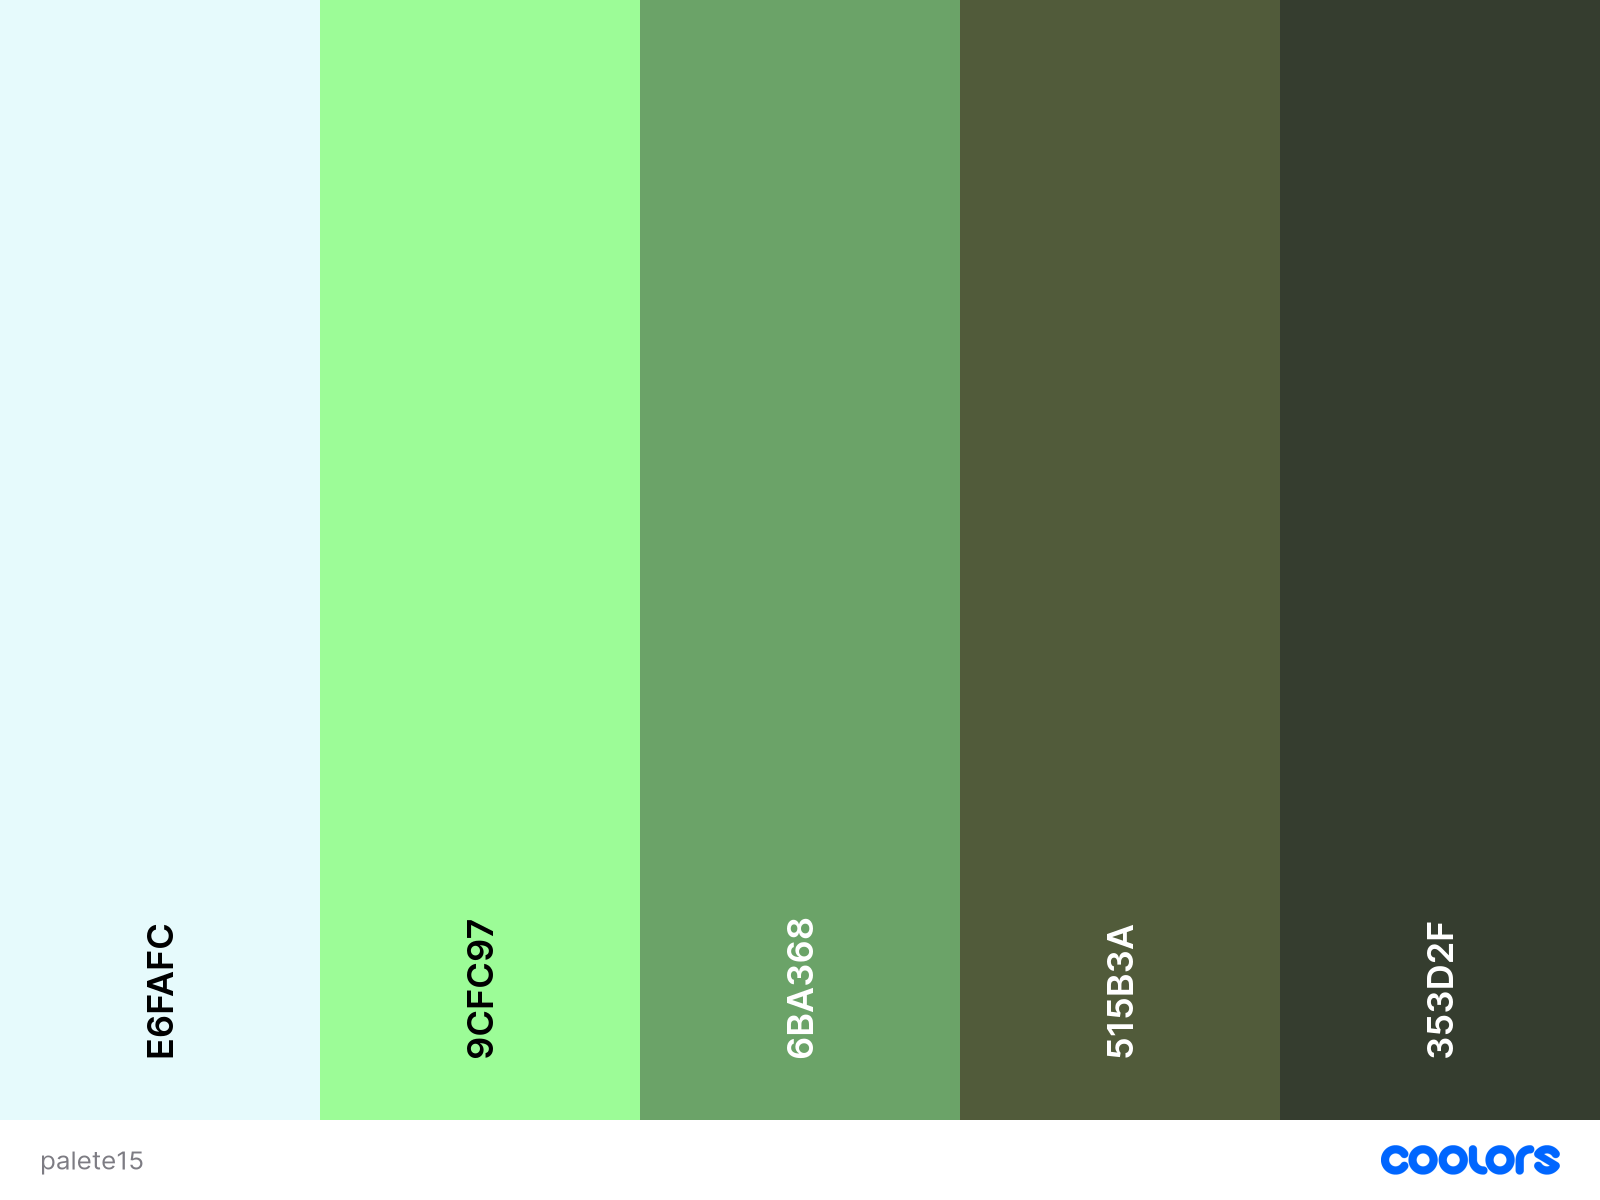
\includegraphics[width=.33\textwidth]{palete15.png}
    }\hfill
    \subfloat[Palette 16]{
        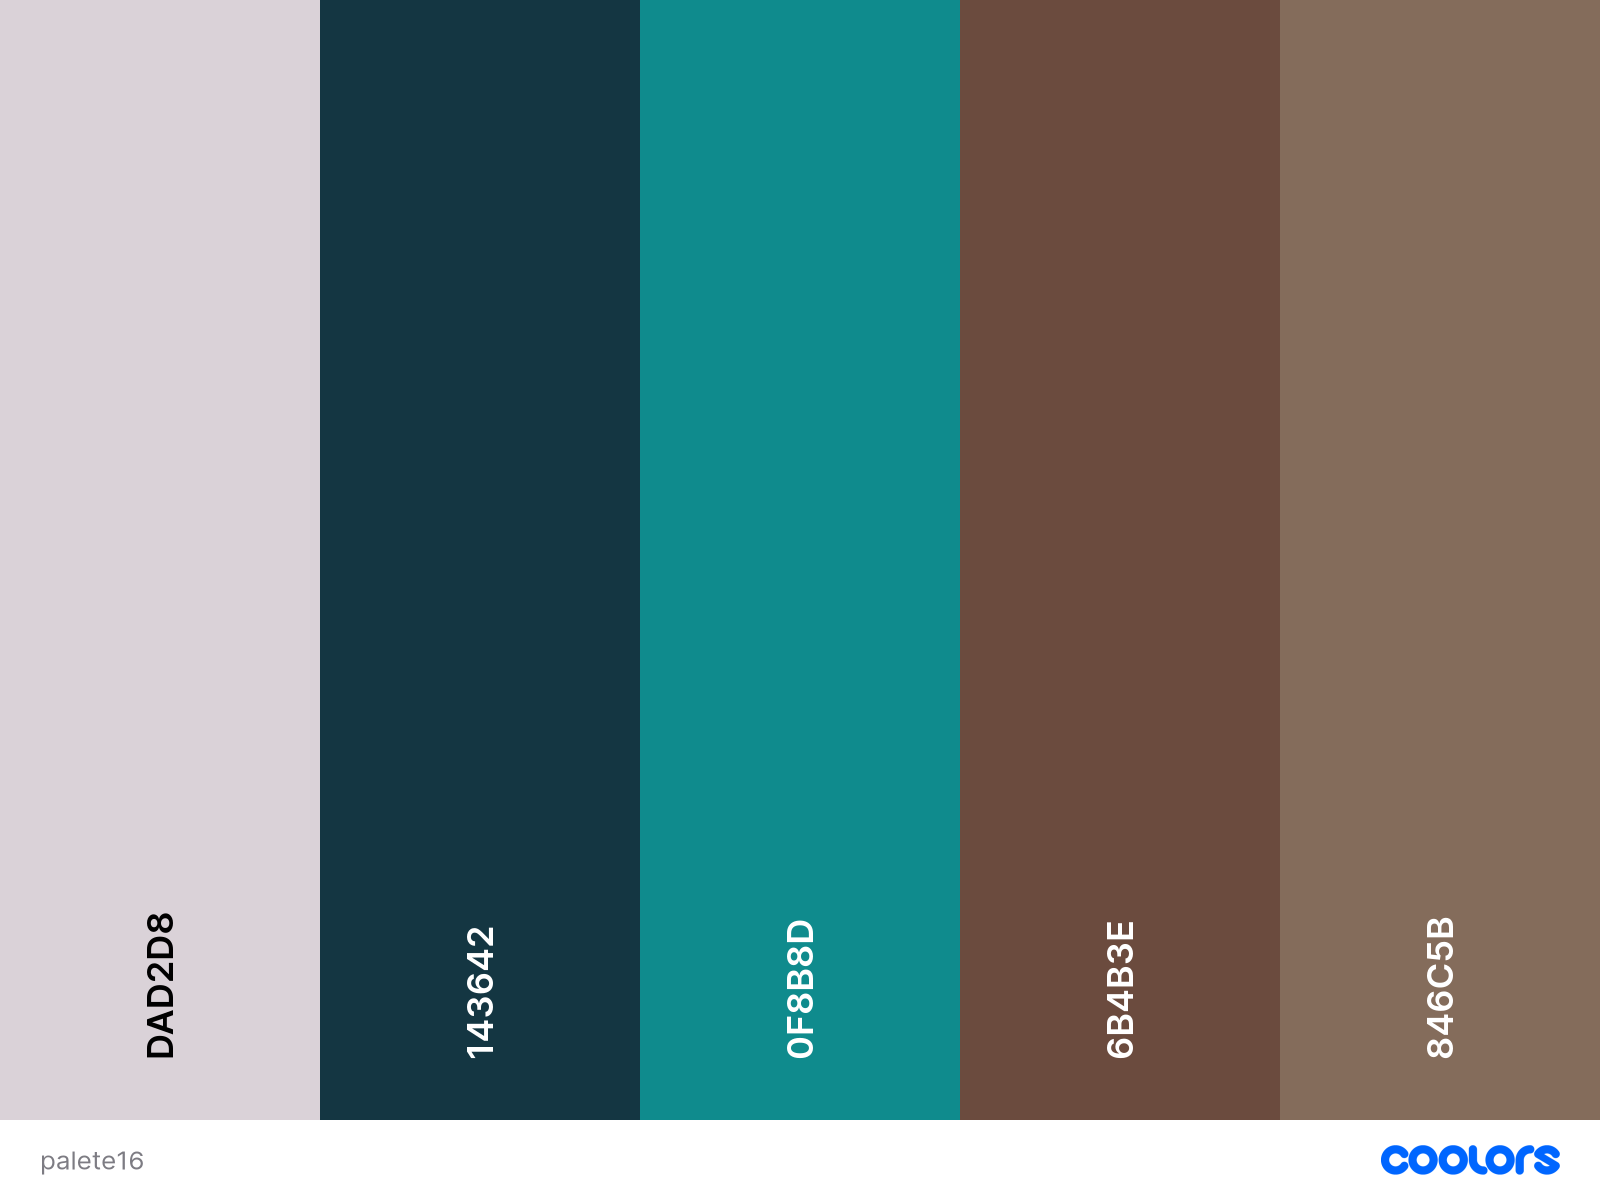
\includegraphics[width=.33\textwidth]{palete16.png}
    }%
    }
\end{figure}
\begin{figure}[H]\ContinuedFloat
    \centerline{%
    \subfloat[Palette 17]{
        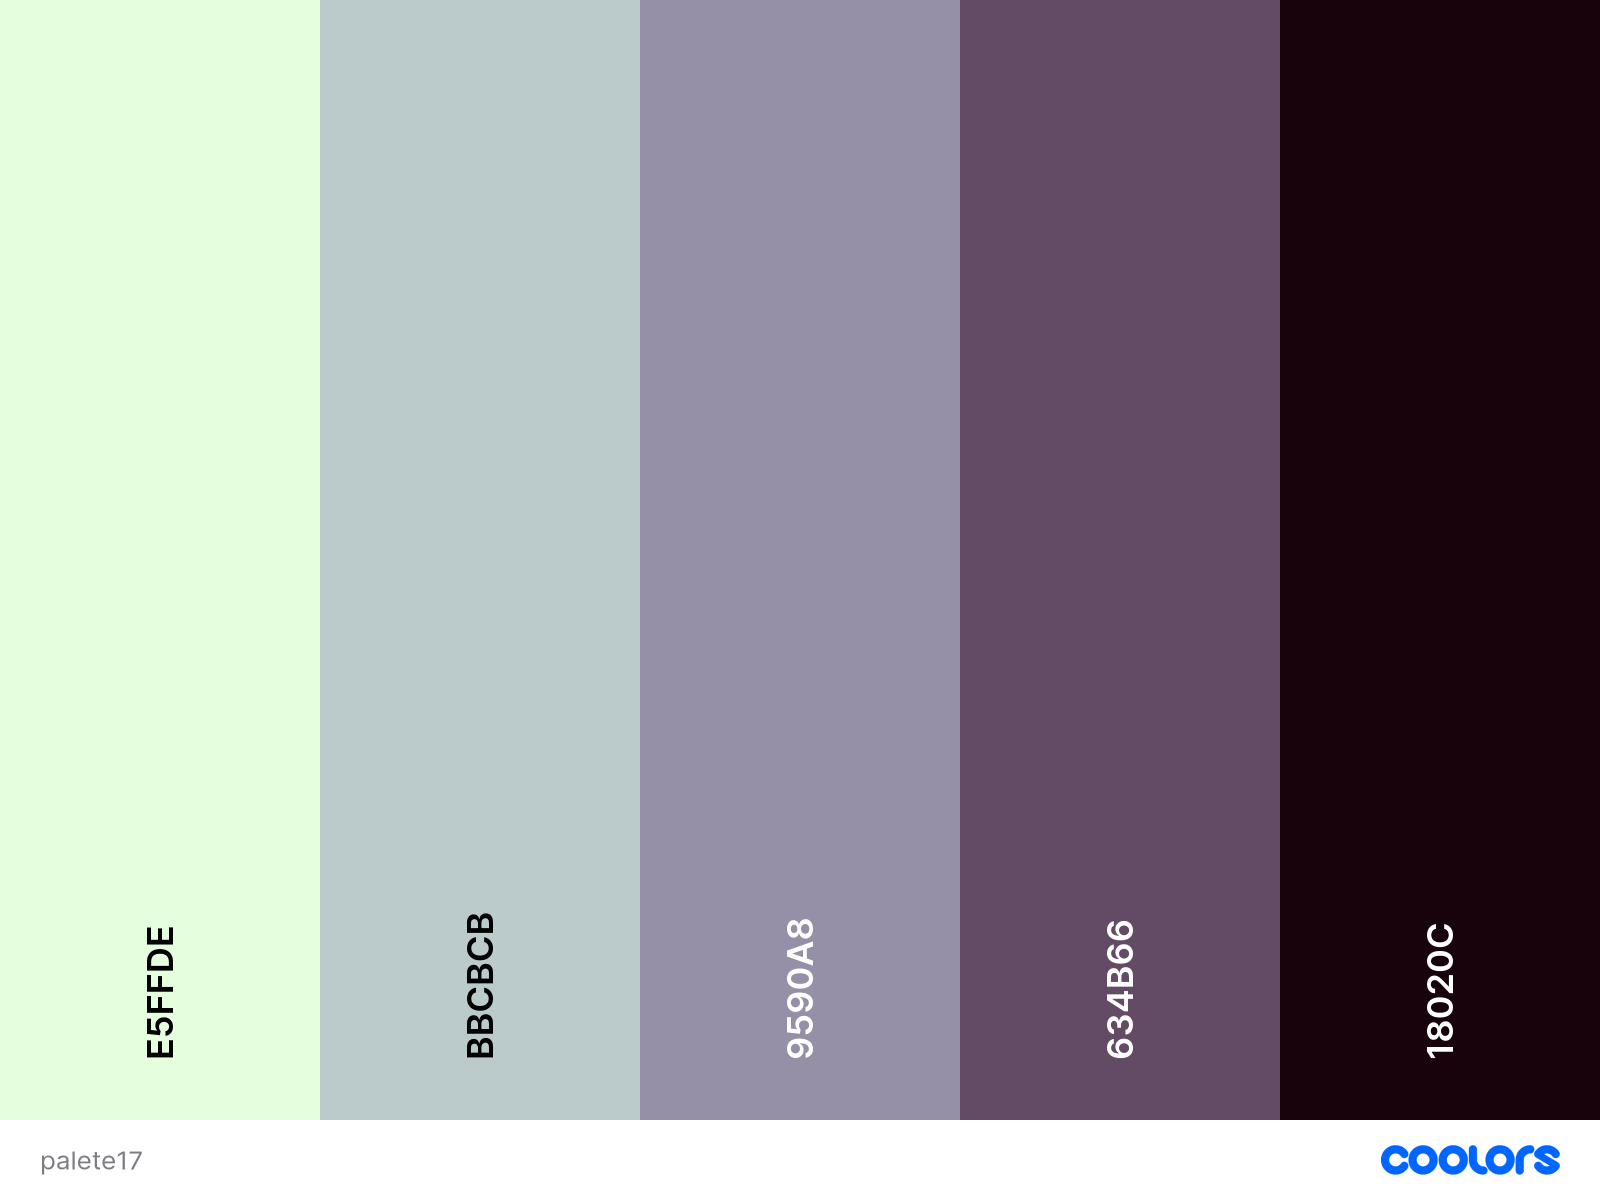
\includegraphics[width=.33\textwidth]{palete17.png}
    }\hfill
    \subfloat[Palette 19]{
        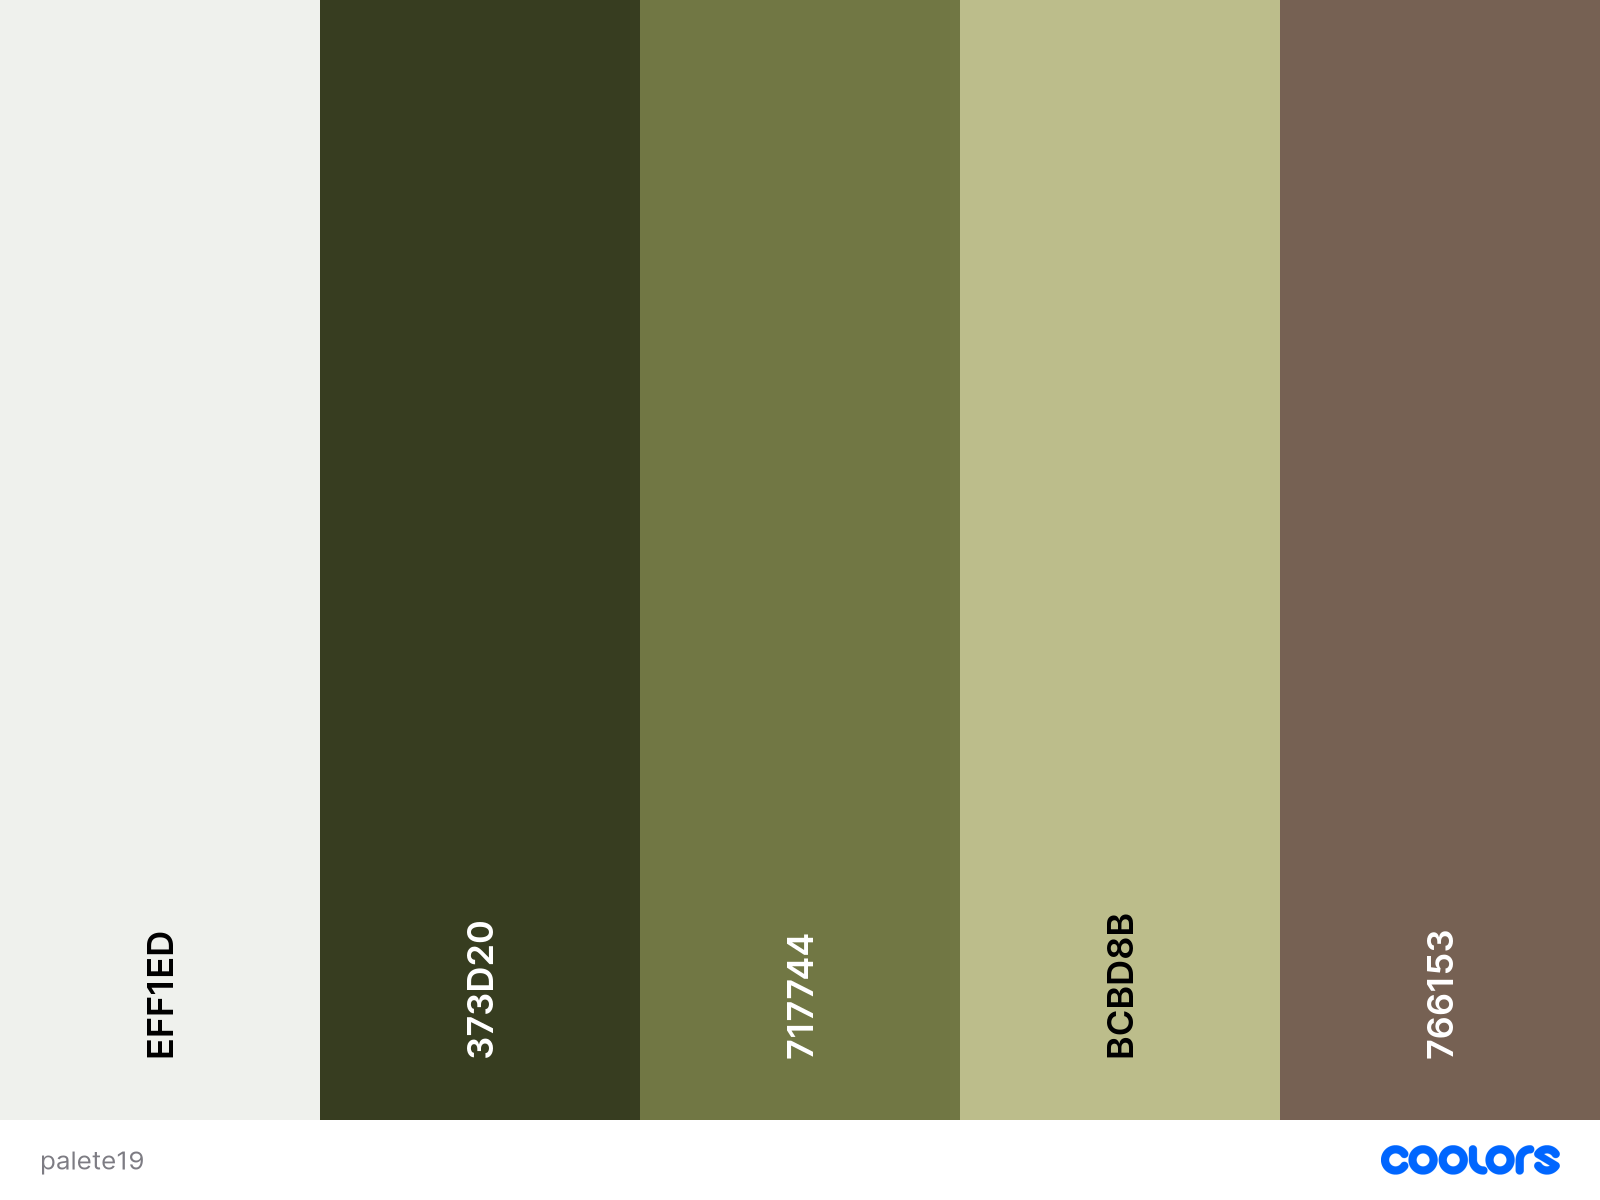
\includegraphics[width=.33\textwidth]{palete19.png}
    }\hfill
    \subfloat[Palette 20]{
        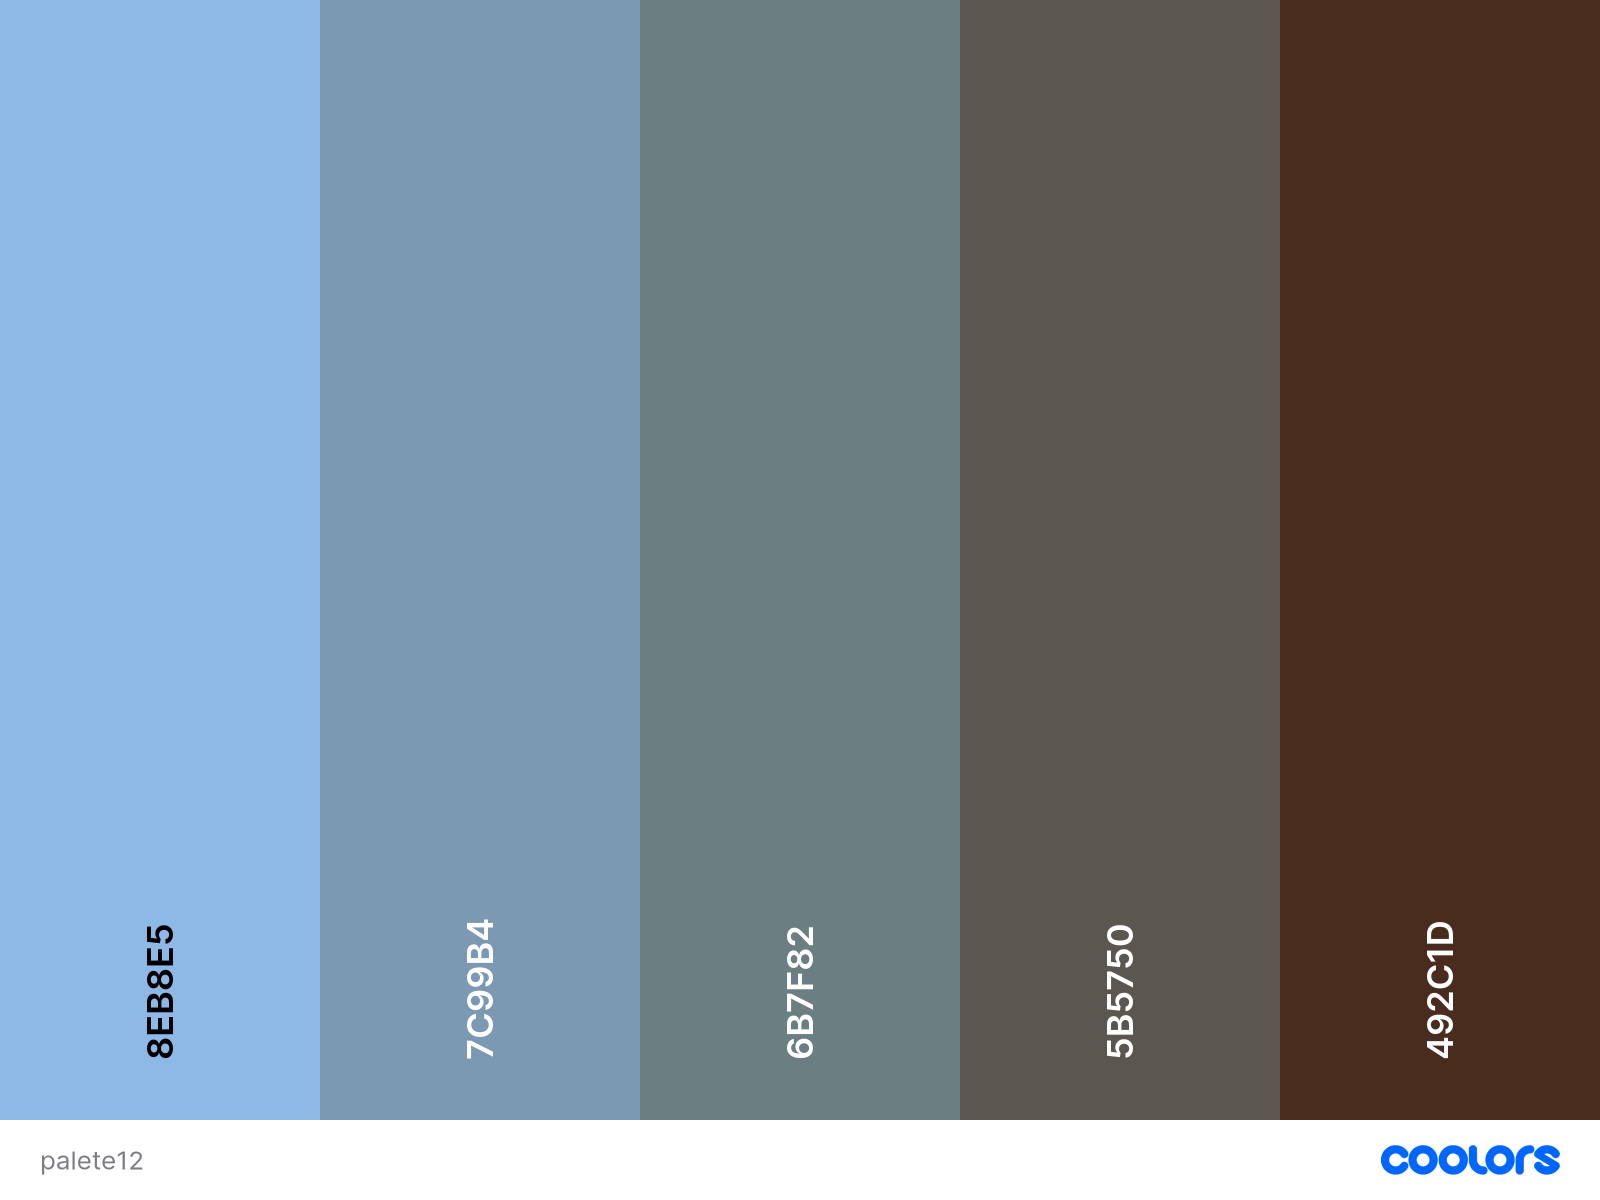
\includegraphics[width=.33\textwidth]{palete20.png}
    }%
    }
    \centerline{%
    \subfloat[Palette 21]{
        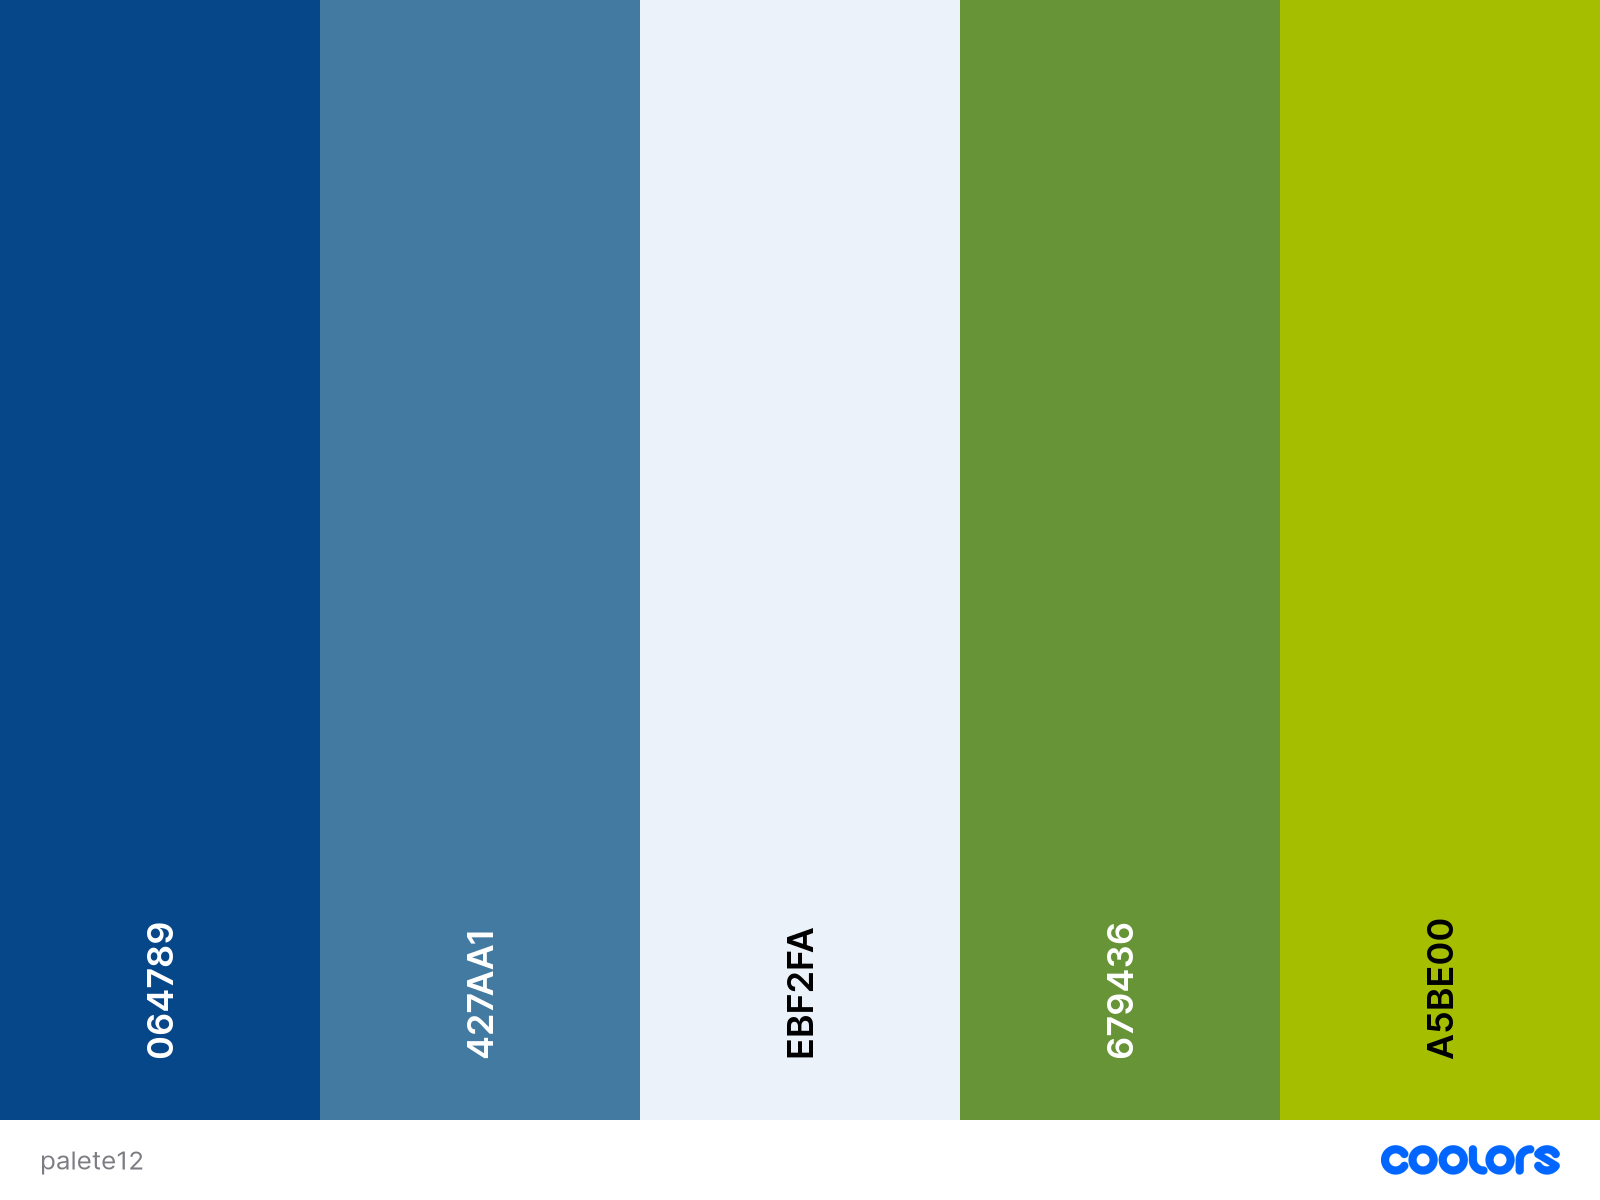
\includegraphics[width=.33\textwidth]{palete21.png}
    }%
    }
    \caption{All the Colour Palettes Generated}
\end{figure}
Subsequently, each member of the group selected their 
five preferred palettes, as illustrated in the 
subsequent table.
\begin{table}[H]
    \centerline{%
        \begin{tabular}{l|*5{c}}
            & \multicolumn{5}{c}{Selected Palletes} \\ 
            \hline 
            Helena & 1 & 5 & 6 & 10 & 20 \\
            Rui & 3 & 6 & 10 & 15 & 19 \\ 
            Sérgio & 4 & 5 & 10 & 16 & 19 \\ 
            Tomás & 3 & 5 & 10 & 15 & 20 \\
        \end{tabular}%
    }
    \caption{Selected Palletes by Each Element of the Group}
\end{table}
Consequently, the colour palettes were ranked as 
follows: Palette 10 received four votes, while Palette 
5 received three. Additionally, Palettes 3, 6, 15, 19,
and 20 were each assigned two votes. \par 
\begin{figure}[H]
    \centerline{%
    \subfloat[Palette 3]{
        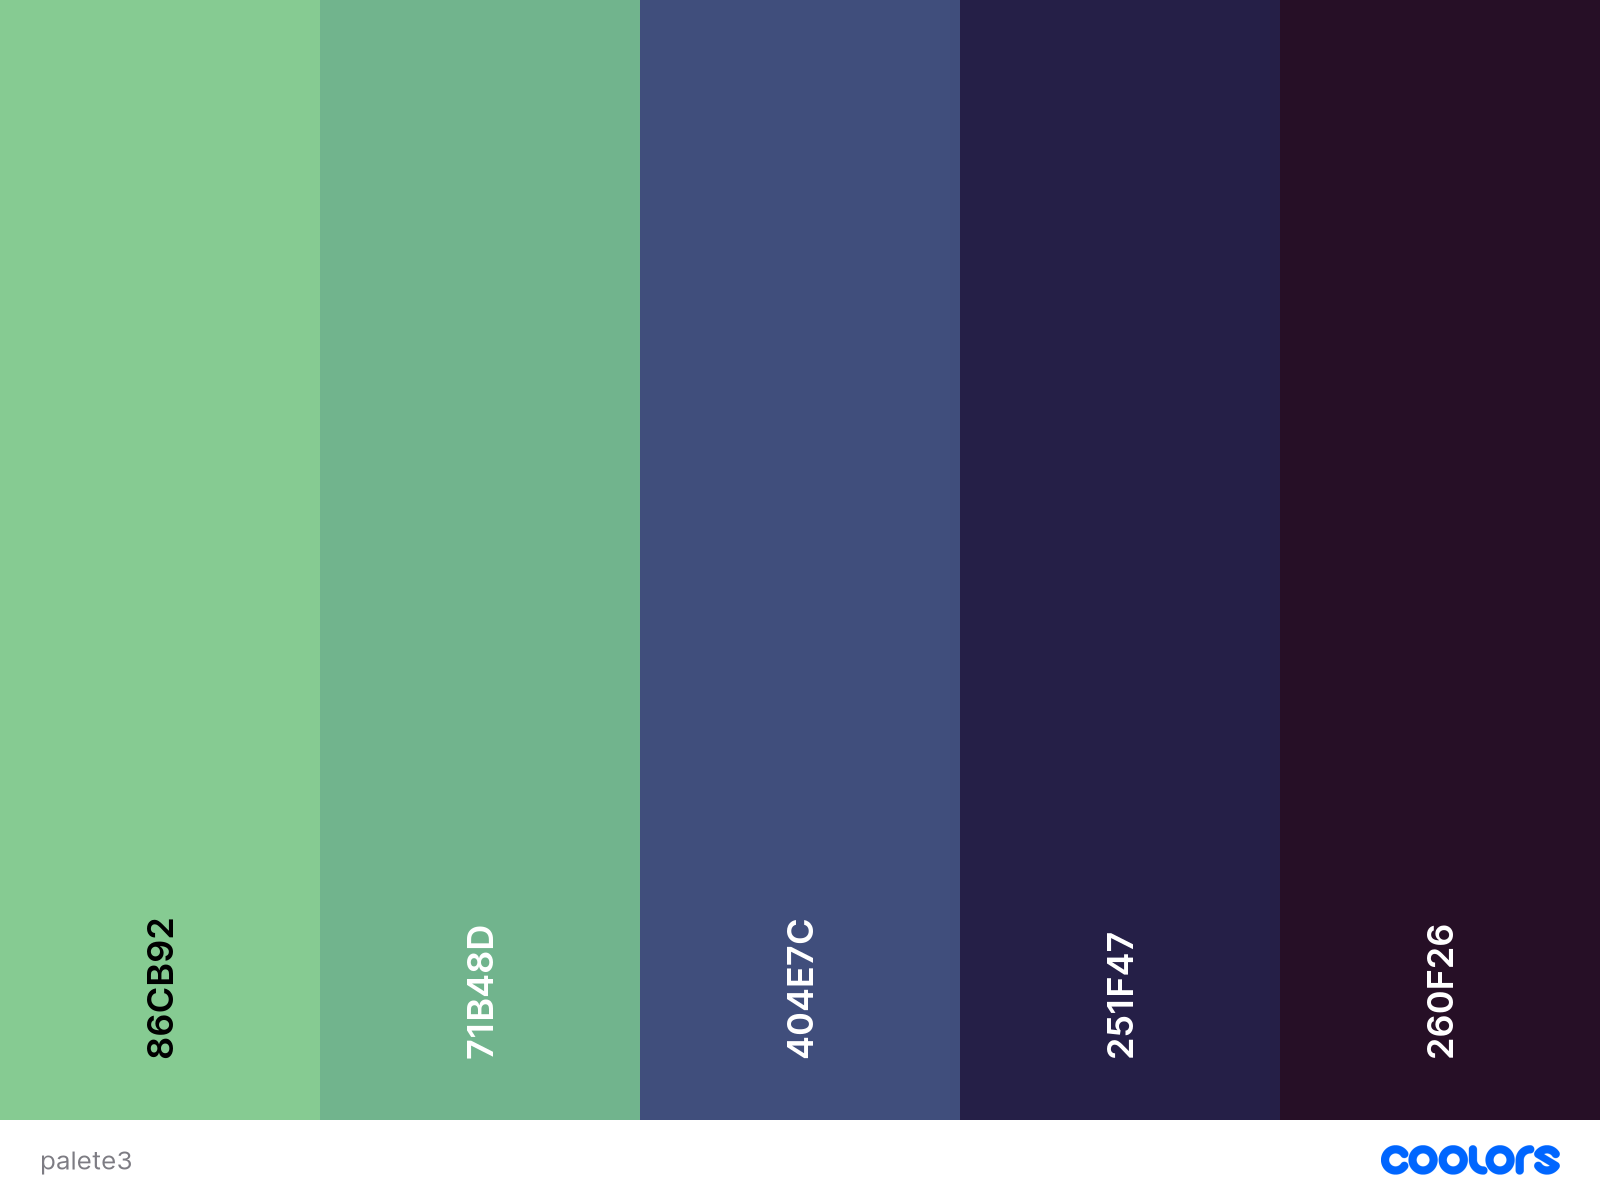
\includegraphics[width=.33\textwidth]{palete3.png}
    }\hfill
    \subfloat[Palette 6]{
        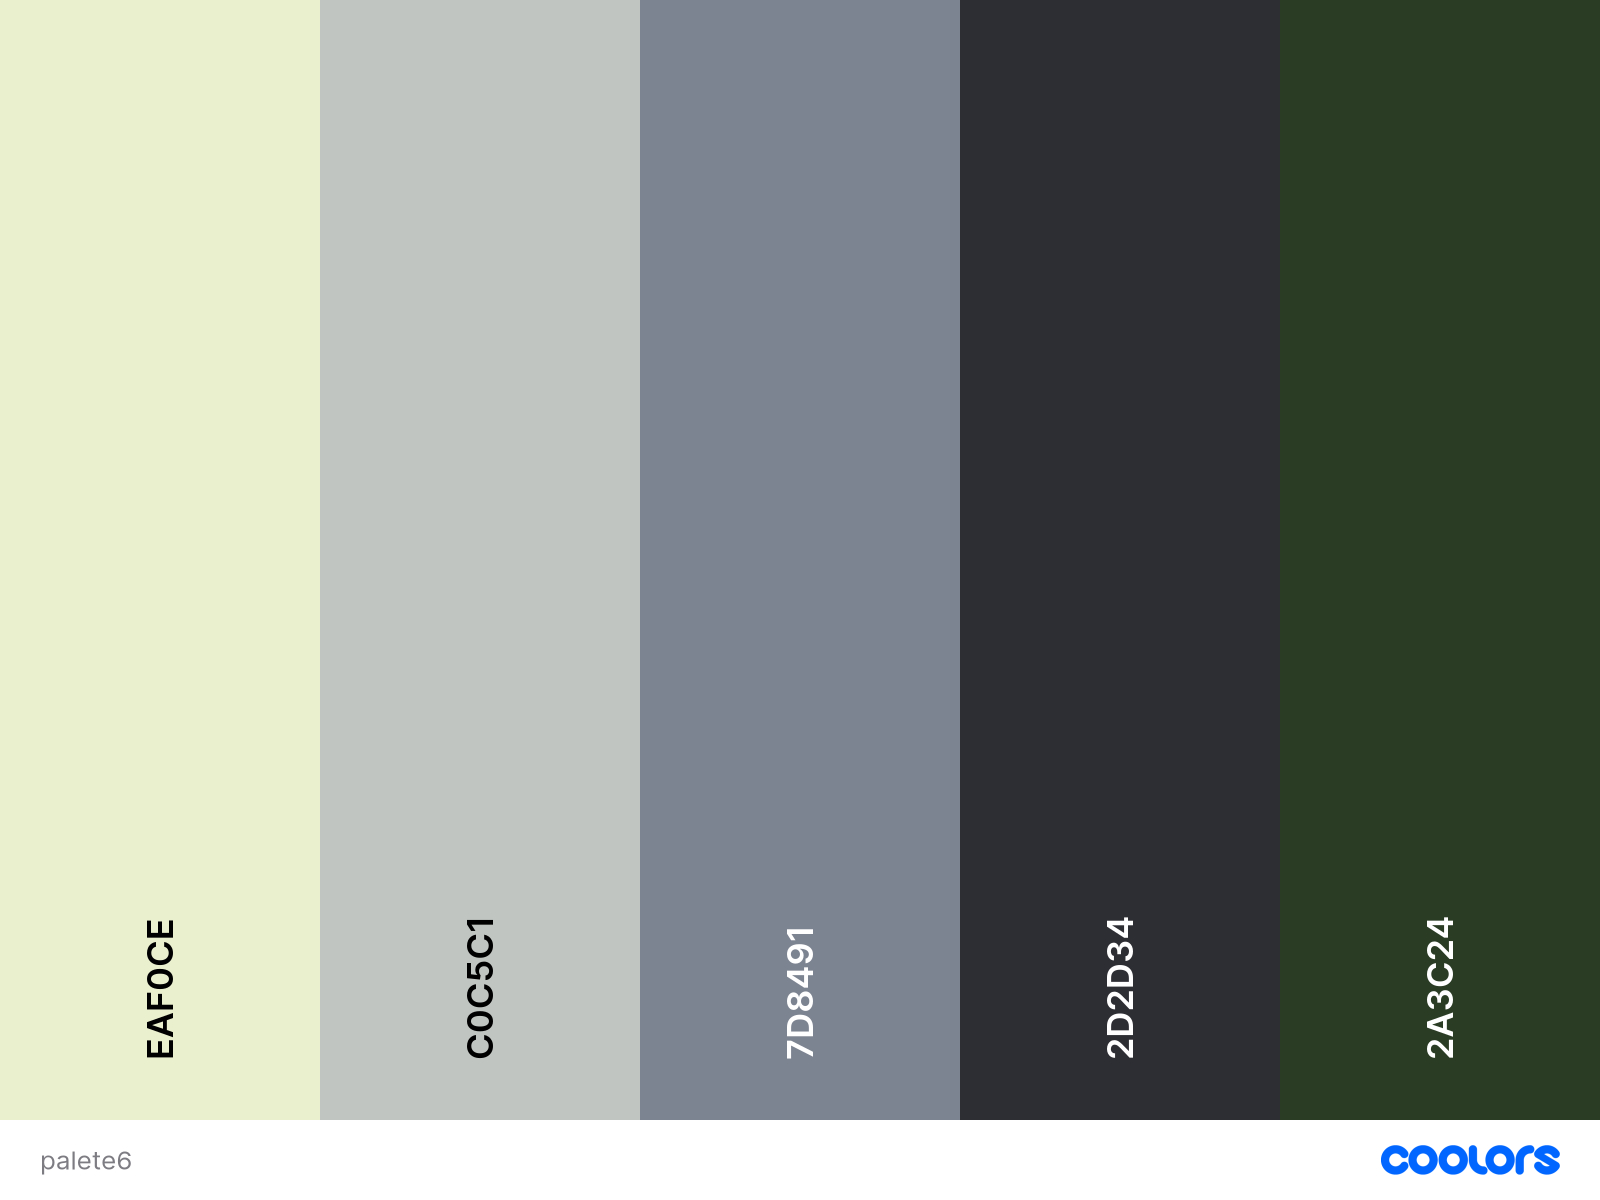
\includegraphics[width=.33\textwidth]{palete6.png}
    }\hfill
    \subfloat[Palette 15]{
        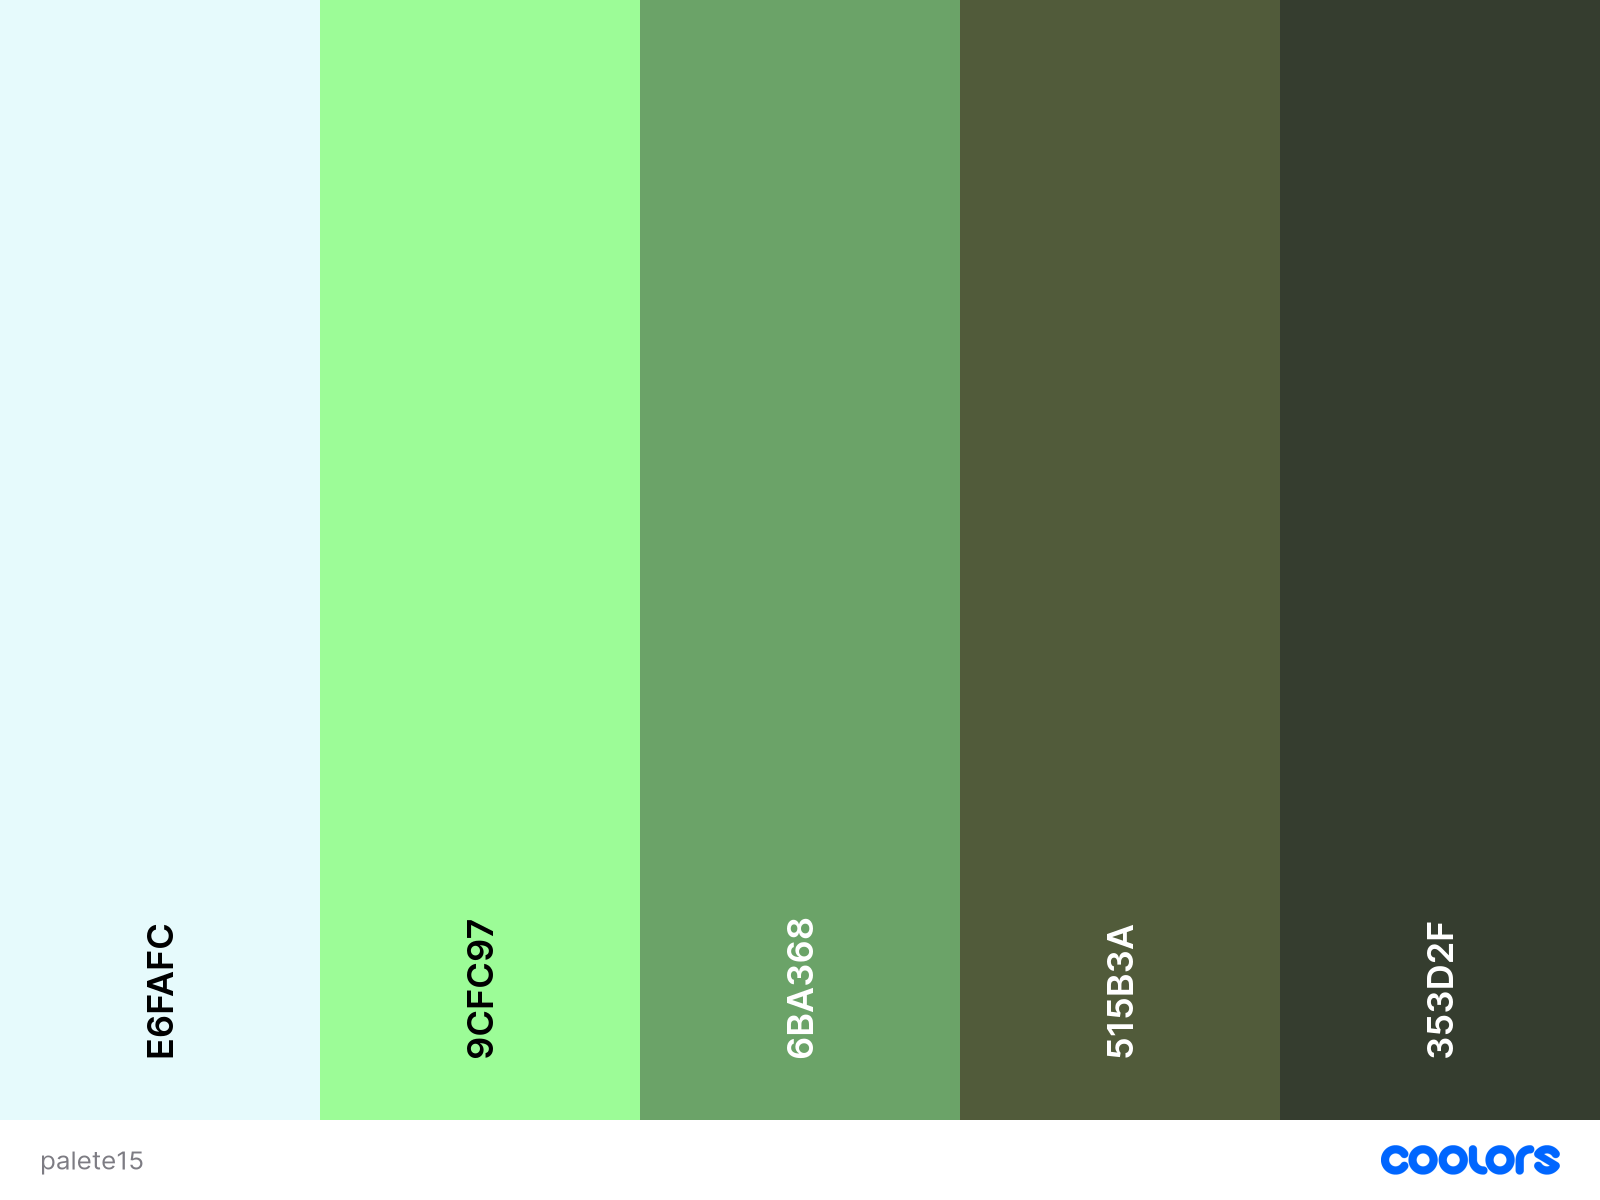
\includegraphics[width=.33\textwidth]{palete15.png}
    }%
    }
\end{figure}
\begin{figure}[H]\ContinuedFloat
    \centerline{%
    \subfloat[Palette 19]{
        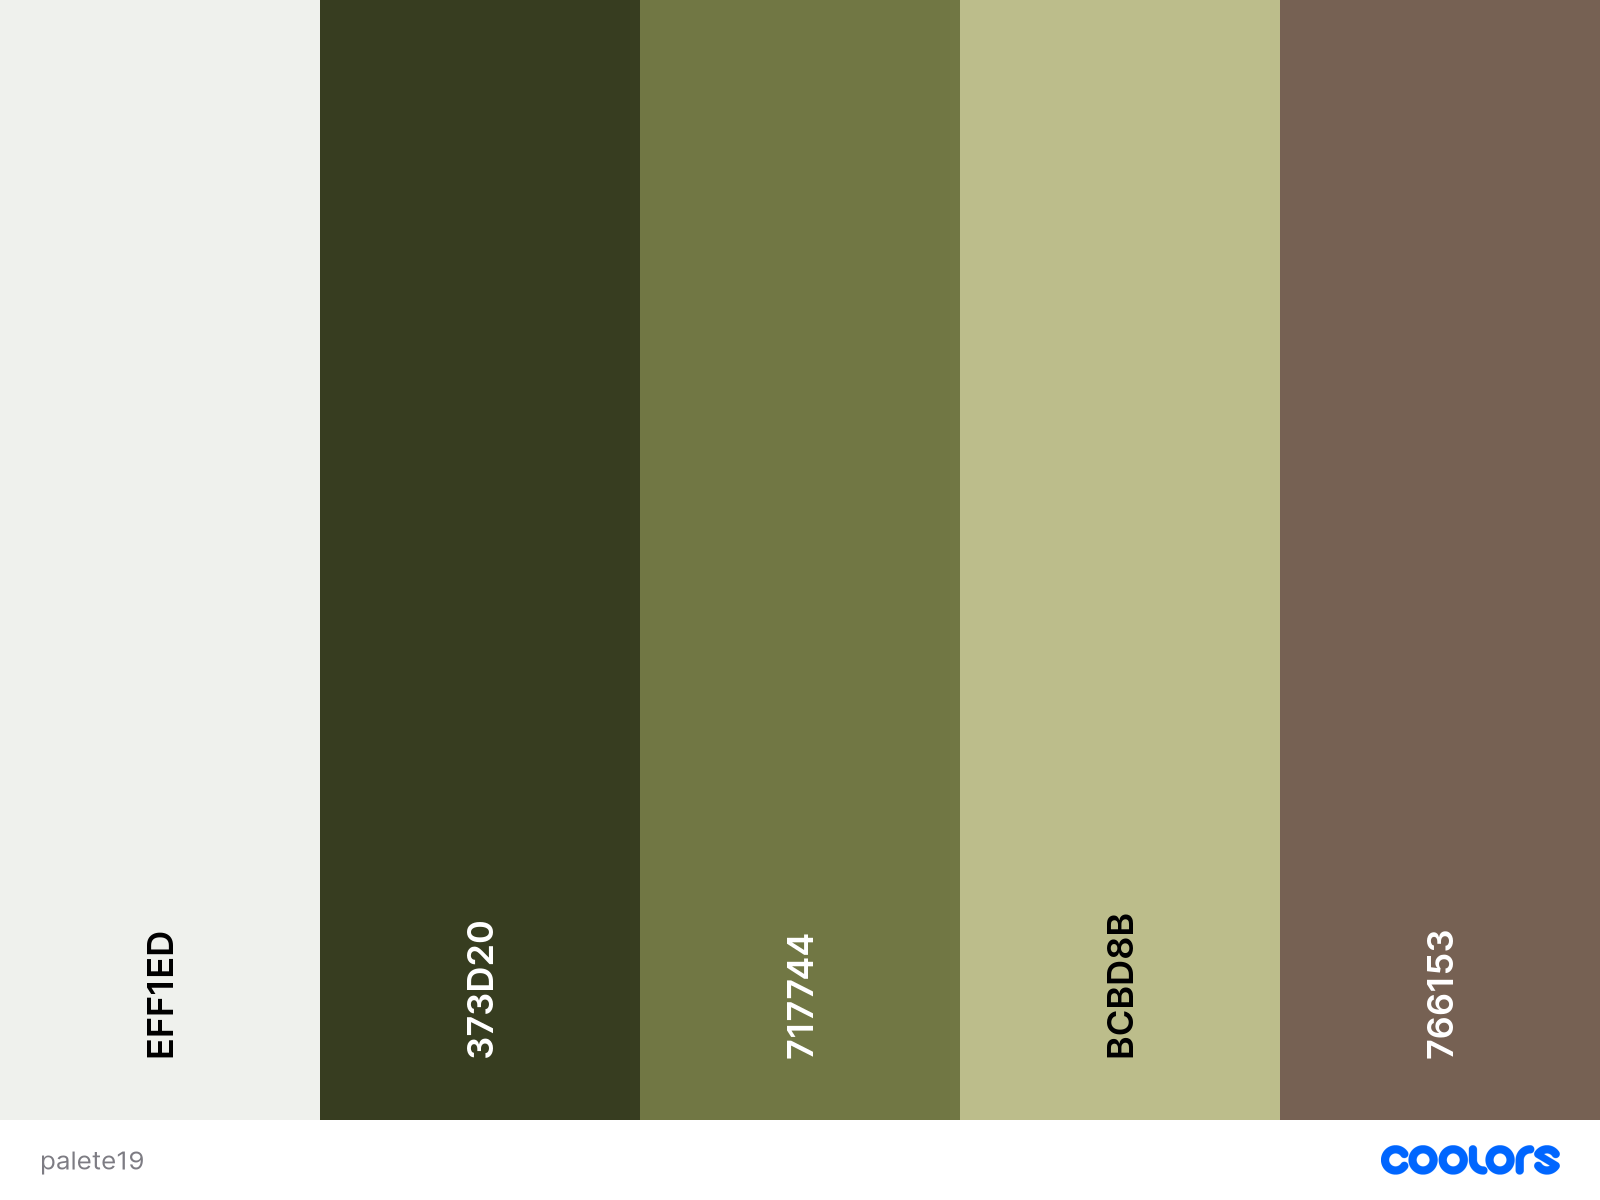
\includegraphics[width=.33\textwidth]{palete19.png}
    }%\hfill
    \subfloat[Palette 20]{
        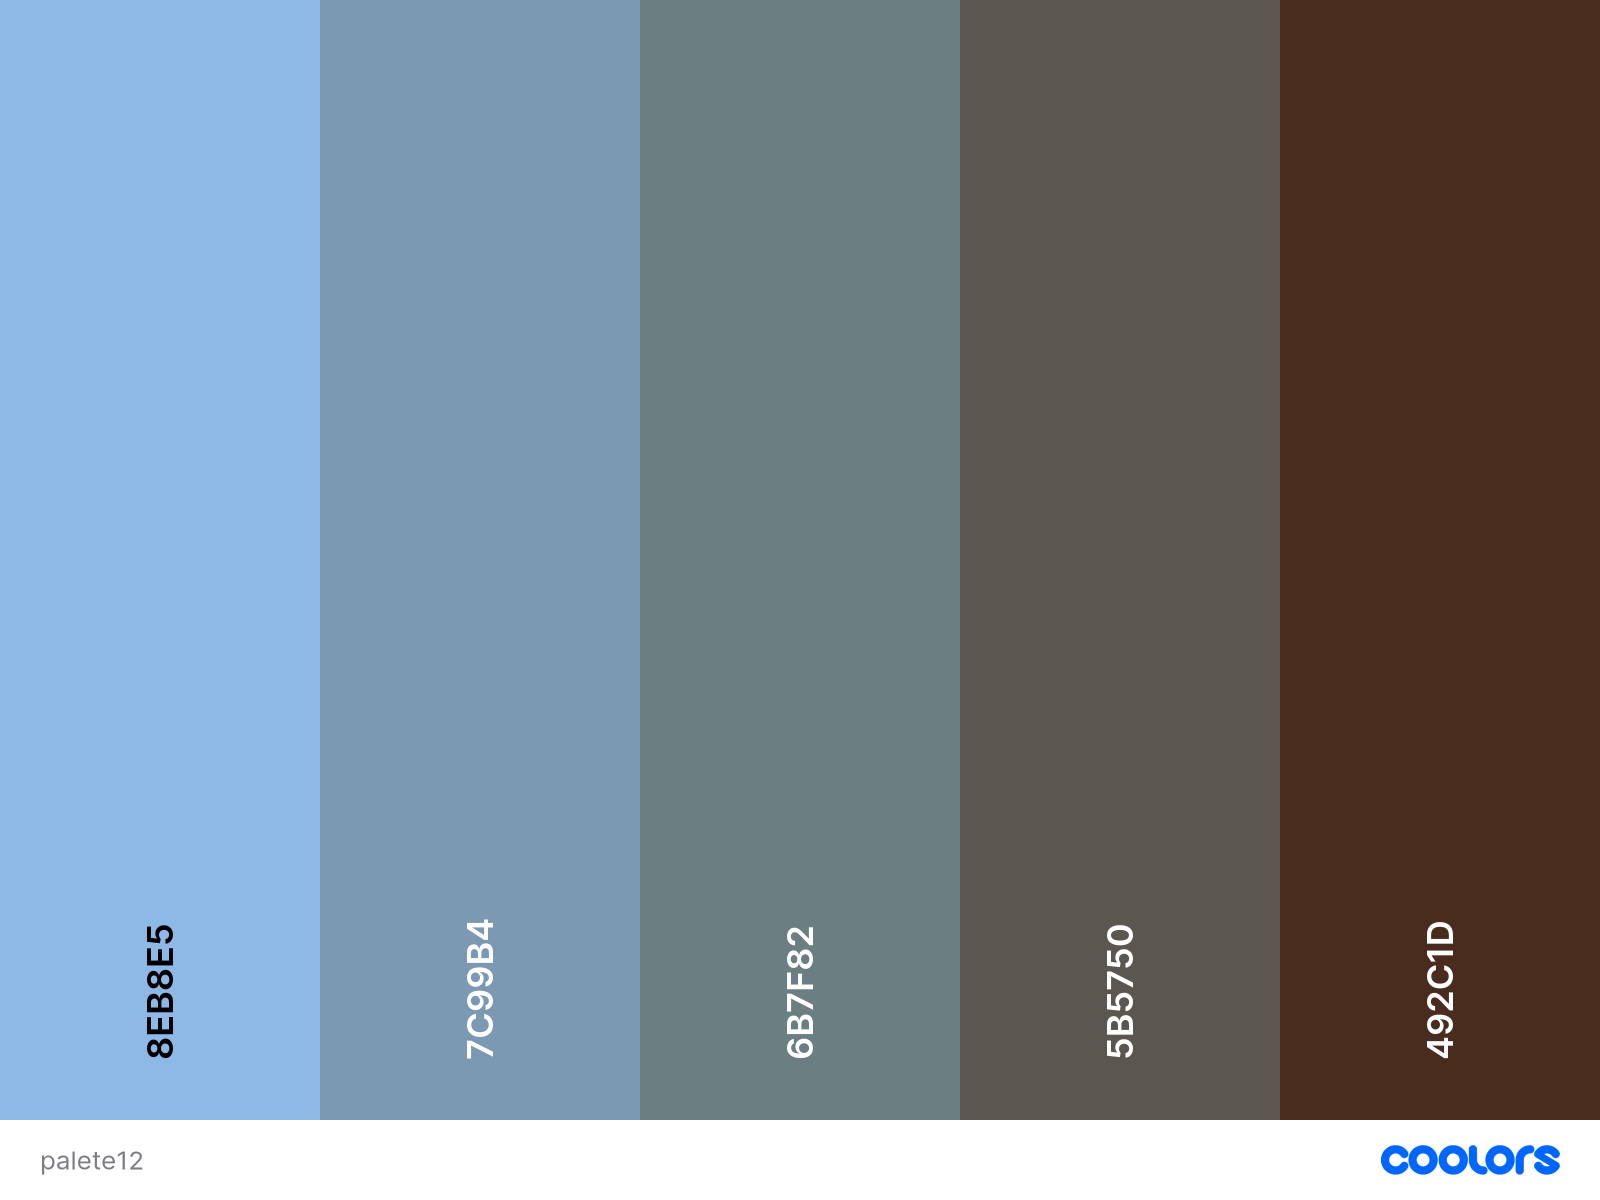
\includegraphics[width=.33\textwidth]{palete20.png}
    }%
    }
\end{figure}
To determine our top three selections, we employed the 
use of Microsoft Forms as a means of conducting a 
tiebreaker between the five palettes that were 
previously presented. To that end, we proceeded to 
order five palettes, with the understanding that the 
number five is the most preferred, followed by four, 
and so on. The results of this process are as follows:
\begin{table}[H]
    \centerline{% 
    \begin{tabular}{l|c|c|c|c|c}
        & Pallete 3 & Pallete 6 & Pallete 15 & Pallete 19 & Pallete 20 \\ 
        \hline 
        Helena & 5 & 3 & 1 & 2 & 4 \\
        Rui & 4 & 2 & 3 & 1 & 5 \\ 
        Sérgio & 3 & 4 & 5 & 2 & 1 \\ 
        Tomás & 5 & 2 & 3 & 4 & 1 \\
        \hline  
        \textbf{Total} & \textbf{17} & \textbf{11} & \textbf{12} & \textbf{9} & \textbf{11}
        \end{tabular}%
    }
    \caption{Tiebreakers Between Palettes in 3\ts{rd} place from the Previous Voting}
\end{table} 
Palette 3 was therefore the most highly rated, thus 
forming the basis of our top three, which includes the 
following paletts: Palette 10, Palette 5 and Palette 3.
\begin{figure}[H]
    \centerline{%
    \subfloat[Palette 10 - First ranked]{
        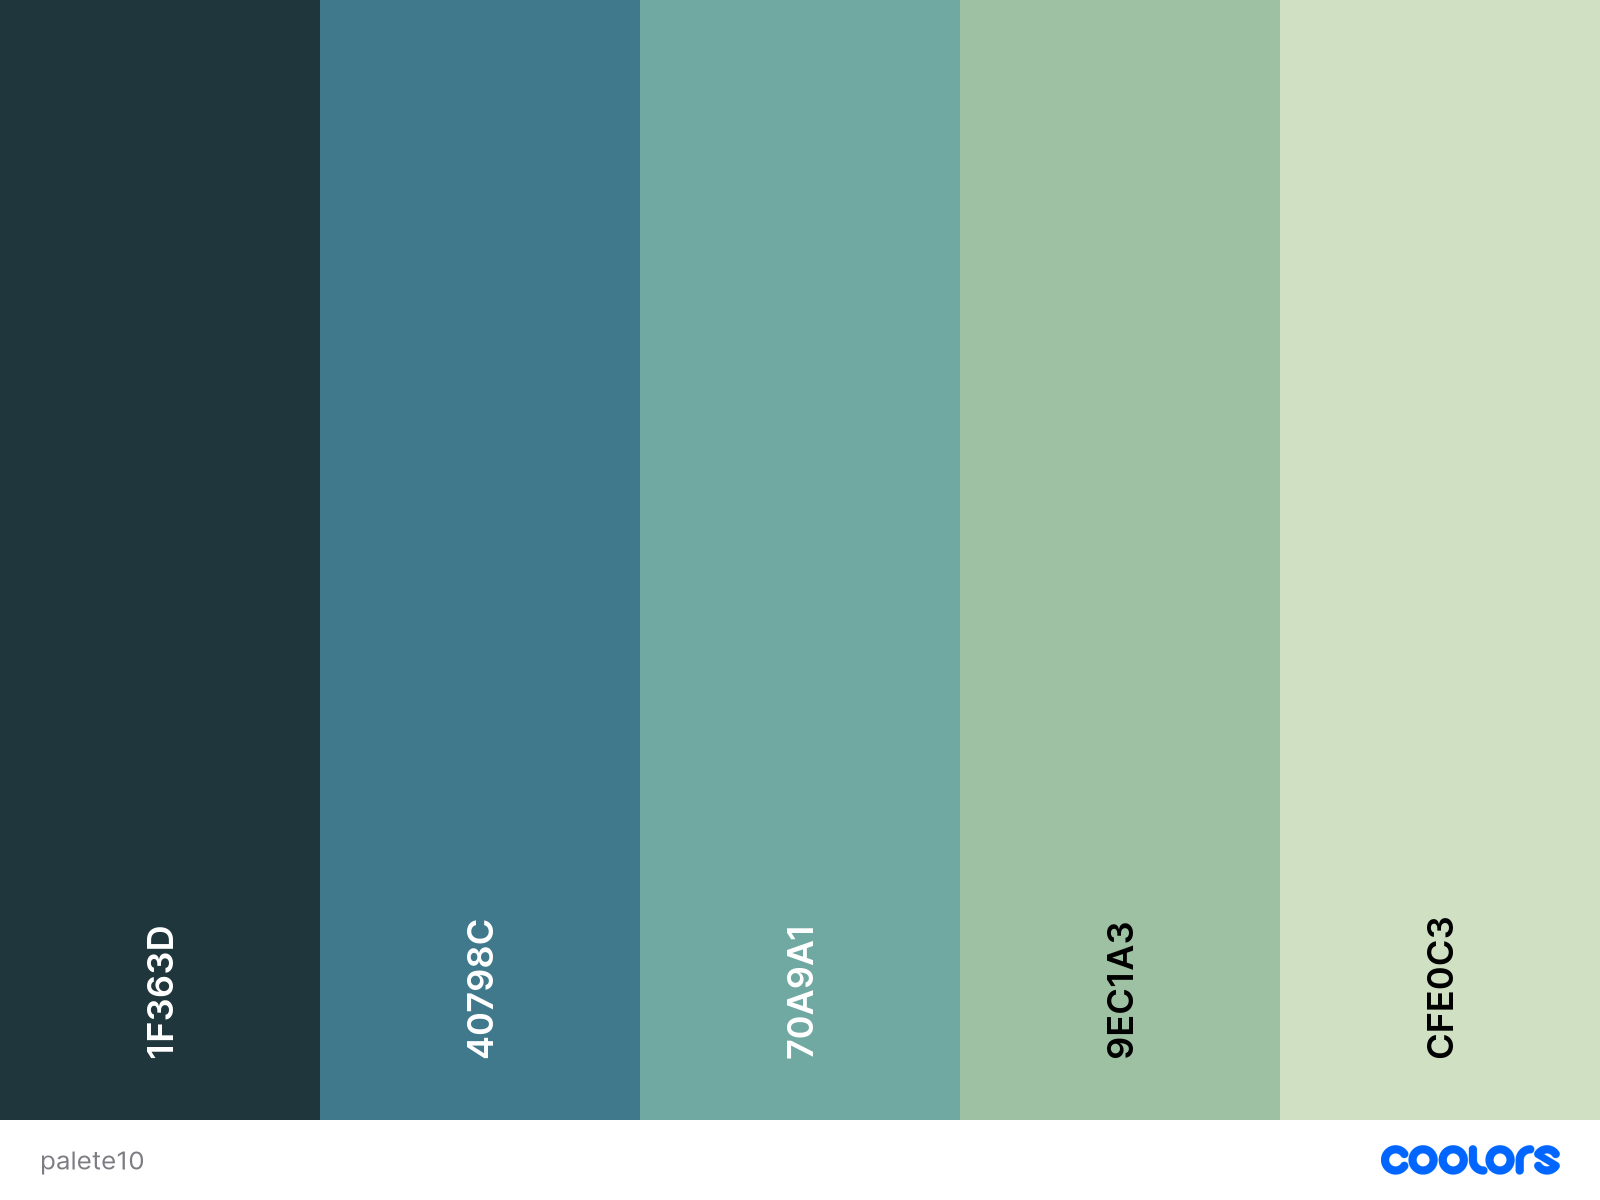
\includegraphics[width=.33\textwidth]{palete10.png}
    }\hfill
    \subfloat[Palette 5 - Second ranked]{
        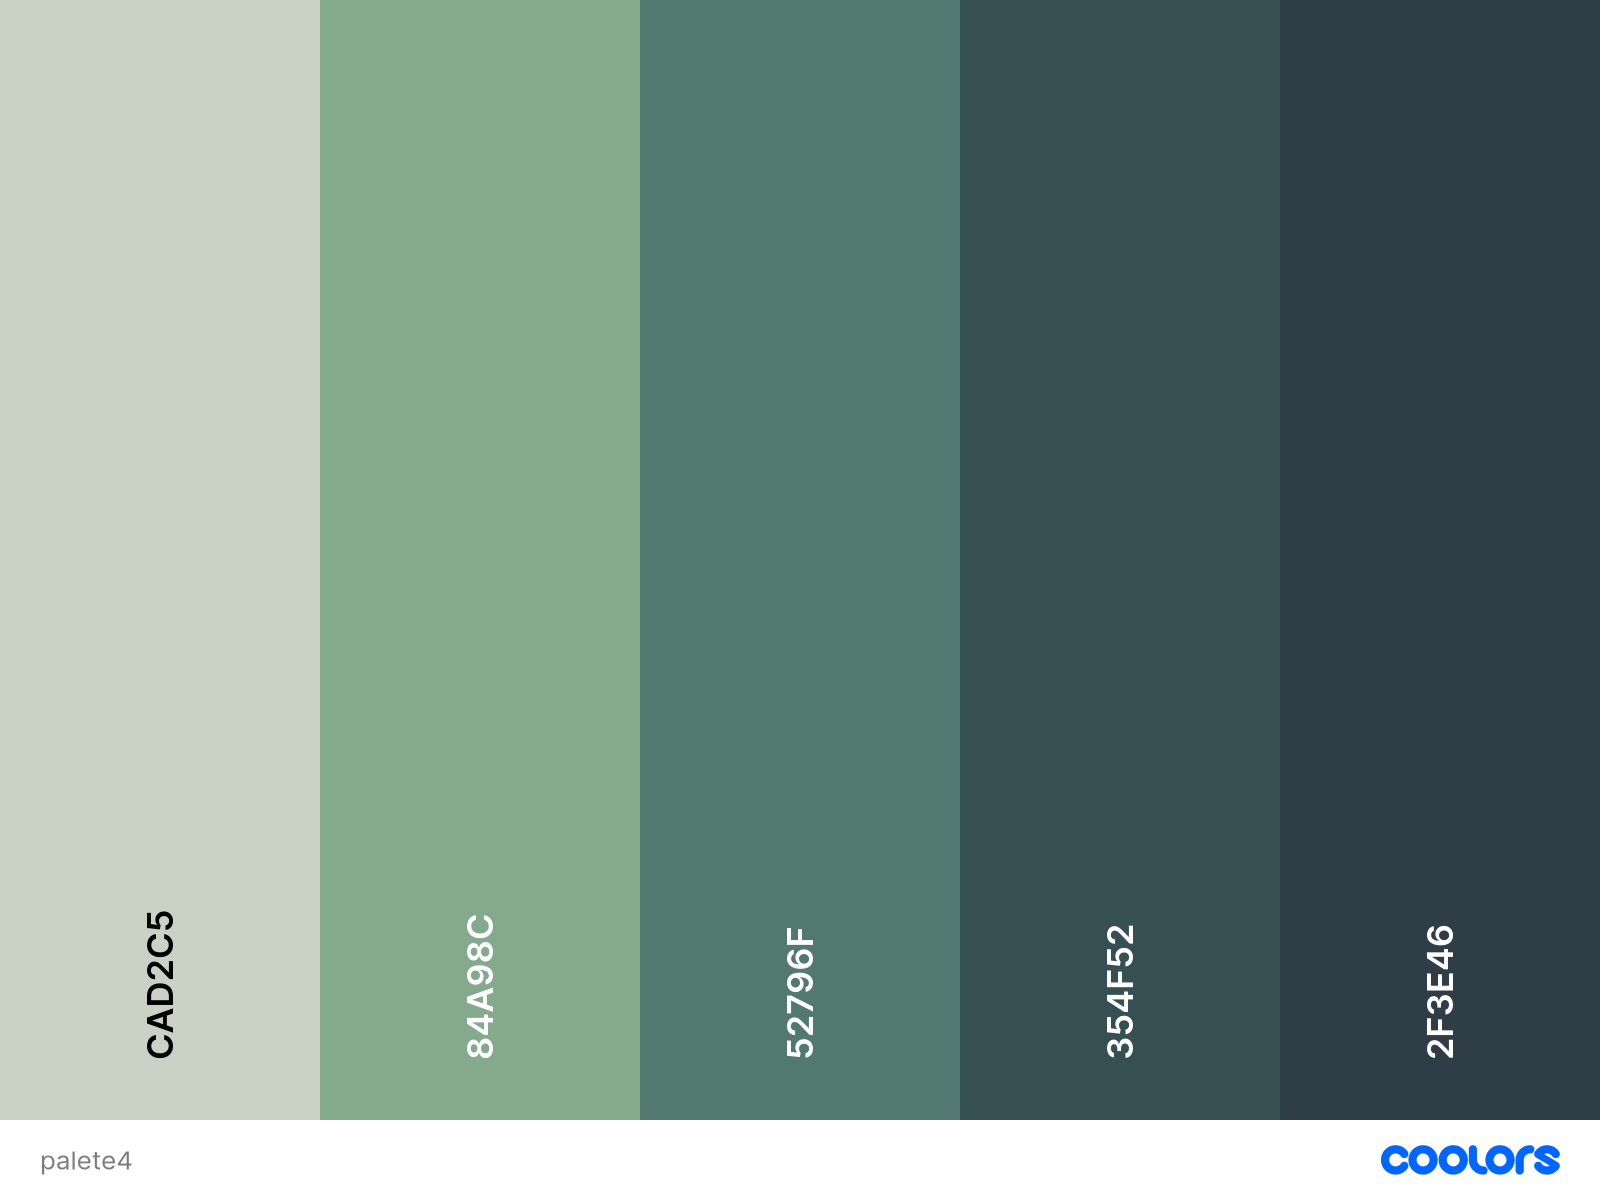
\includegraphics[width=.33\textwidth]{palete5.png}
    }\hfill
    \subfloat[Palette 3 - Third ranked]{
        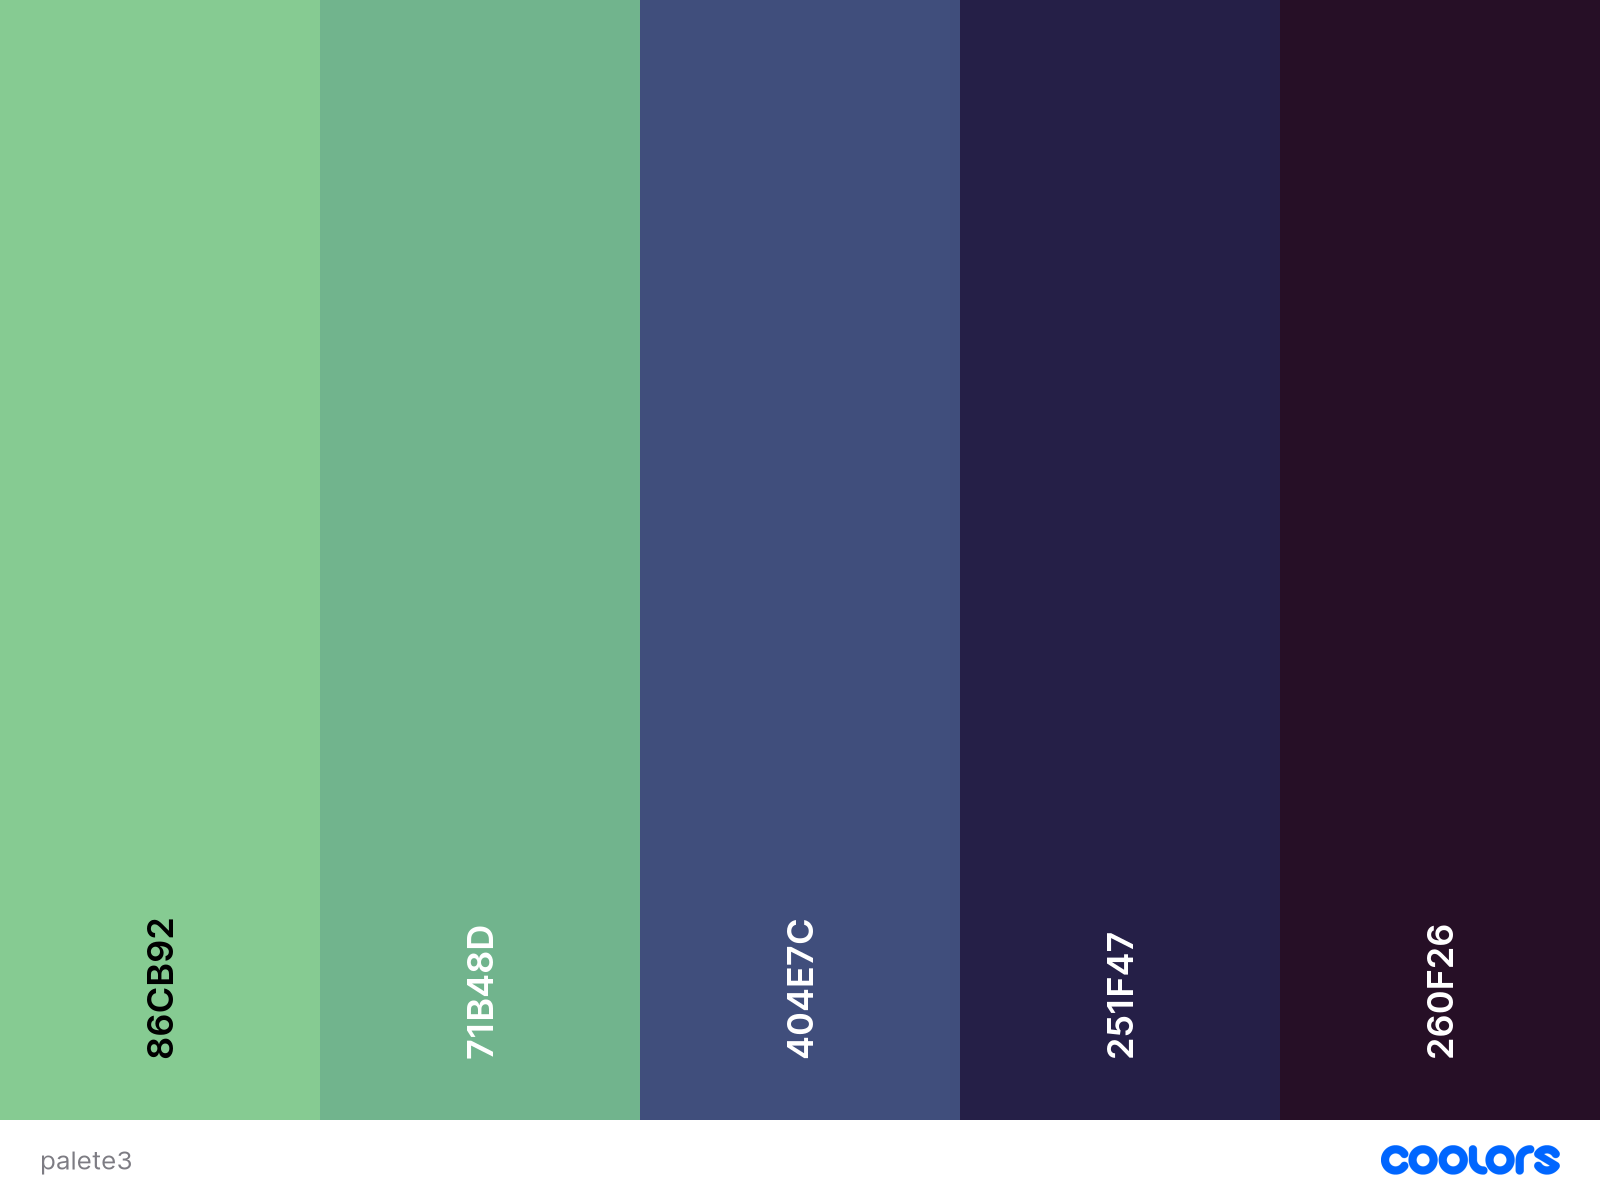
\includegraphics[width=.33\textwidth]{palete3.png}
    }%
    }
    \caption{The Three Highly Ranked Palettes}
\end{figure} 
After all of these rankings were done, we then borrowed the 
color codes of the first ranked palette, Palette 10 as we mentioned 
(1F363D, 40798C, 70A9A1, 9EC1A3 and CFE0C3) and used them 
in Figma (\url{https://www.figma.com}), a web application focused on user interface 
(UI) and user experience (UX) design, in order to replicate 
the dashboard shown in \ref{dashboard}.
\section{Improvements}
As we were developing the final dashboard which will be 
discussed in \ref{description}, we felt the need to add 
new colors to the chosen palette, like EFFFE3, 
due to certain conflicts with the map.
\section{Description of the Visible System Components} \label{description}
So, the final dashboard is made up of the following: 
\begin{itemize}
    \item Log Panel: showcases real-time alerts
    \item Map: 
    \item Resources Panel: enlists the number of resources 
    available on the chosen local area
    \item Situation Panel: has the sensors's status
    \item Cameras Panel: gives the user the possibility 
    to alternate between camera angles
\end{itemize}